\part{Social Fabric Project}
\label{part:social_fabric}
\chapter[Data Extraction]{Phone Activity and Quantitative Data Extraction}
\initial{T}{he} main objective of part \ref{part:social_fabric} of this thesis is to investigate behavioural patterns in the phone activities of the participants in the Social Fabric Project, and to predict various traits of the users based only on their phone logs. Throughout the part, I'll provide brief examples of usage for the software I've written to process the large amount of data available and to apply various prediction schemes to it, while the source code itself is included in the appendix.

My first objective was to investigate how various phone activities correlate with each other temporally, i.e. how a given user's probability for e.g. receiving a call increases or decreases around other activities such as moving around physically. This is the topic of section \ref{sec:activity_triggers}.

Next, I set out to replicate some recent research results\todo{kilder!!!} claiming that people's phone activities predict certain psychological traits. In the most general terms, then, the task consists of predicting a collection of numbers or labels denoted $Y$ based on a set of corresponding data points $X$. The topic of section \ref{sec:data_extraction} is the extraction of the many-dimensional data points or \textit{feature vectors} $X$ from the phone logs of the participants, while section \ref{sec:output_data} gives a brief description of the psychological traits $Y$. Finally, section \ref{sec:LDA} derives an often used linear classification method known as Linear Discriminant Analysis or Fisher's Discriminant and provides a discussion of why it fails for the present dataset, which serves to motivate the more sophisticated prediction schemes introduced in chapter \ref{sec:profiling}.

\section{Temporal Correlations in Activity}
\label{sec:activity_triggers}
One category of interesting quantities is the predictability of mobile phone behaviour from recorded behaviour at different times, i.e. the influence of certain events deduced from a user's Bluetooth, GPS or call log data on the tendency of some event to happen in the near past or future. A simple example would be to determine how much placing or receiving a call increases or decreases the probability of a user placing or receiving another call in the period following the first call.

This analysis was performed by comparing an 'activity' signal with a 'background' signal in the following fashion: For each user, the time period around each call is sliced into bins and the each of the remaining calls placed in the bin corresponding to the time between the two calls. Once divided by the total number of calls for the user, this is the activity signal. The background is obtained in a similar fashion but comparing each call in a given user's file with calls in the remaining users' files.

This involves repeatedly binning the time around certain events and then determining in which bin to place other events; a situation in which confusion may arise easily and errors may be hard to identify. To accommodate this, I started out by writing a custom array class designed to greatly simplify the binning procedure. This class called features the following:
\begin{itemize}
	\item Methods to bin the time around a given event and determine determine which bin a given event falls into. This is useful to implement in the class itself as one then avoids having to continually worry about which bin an event fits into, and as it ensures that bin placement errors can only arise in one small piece of code which can then be tested rigorously.
	\item Attributes that keep track of the number of events that didn't fit into any bin, and of the current centre of the array, which can then be manipulated to move the array and a method to use this to return a normalized list of the bins.
\end{itemize}
In short, the binarray can be visualized as a collection of enumerated buckets that can be moved so as to center it on some event and then let other events 'drip' into the buckets. The code for this class is included in \ref{sec:phonetools.py}. In general, objects can be converted to byte streams and stored using Python's pickle module, but as that tends to be both slow and insecure, I generally used json to save my objects. This poses a slight problem as some data types, such as tuples, and custom classes in general are not json serializable. I got around this by writing some recursive helper methods to help store the relevant information about arbitrary nested combinations of some such objects and to help reconstruct said objects again. These are also included in section \ref{sec:phonetools.py}. As an example of usage, the following code constructs a Binarray, centers it around the present time, and generates a number of timestamps which are then placed in the event. It is then saved to a file using the helper method previously described.
\begin{snippet}
	from time import time
	from random import randint
	#Create Binarray with interval +/- one hour and bin size ten minutes.
	ba = Binarray(interval = 60*60, bin_size = 10*60)
	#Center it on the present
	now = int(time())
	ba.center = now
	#Generate some timestamps around the present
	new_times = [now + randint(-60*60, 60*60) for _ in xrange(100)]
	for tt in new_times:
		ba.place_event(tt)
	
	#Save it
	with open('filename.sig', 'w') as f:
		dump(ba, f)
\end{snippet}
This data will be visualized by plotting the relative signal from the activity of some event, such as in- or outgoing calls or texts, over the background (simply $A/B$) around another type of event hypothesized to trigger the activity. 

\subsection{Influence of phone calls}
\label{sec:trigger_phone}
I first investigated the effects of incoming and outgoing calls as triggers for other phone activities. The call logs were stored in a format where each line represents a hashmap with quantities such as call time or call duration mapping to their corresponding value. Below is an example of one such line, were any personal data have been replaced by a random number or hexadecimal string of equal length.
\begin{snippet}
	{
		"timestamp": 6335212287, 
		"number": "c4bdd708b1d7b82e349780ee1e7875caa600c579", 
		"user": "ea42a1dbe422f83b0178d158f154f4", 
		"duration": 483, 
		"type": 2, 
		"id": 45687
	}
\end{snippet}
the text logs are similar except for the missing duration entry. Computing the relative signal in Binarrays centered on each incoming and outgoing call using bin sizes of three and thirty minutes resulted in the plots shown in figures \ref{fig:calls_three_minutes} and \ref{fig:calls_half_hour}, respectively.
\begin{figure} %[htb]
	\centering
	\subbottom[Relative activity of events triggered by incoming calls.]{%
		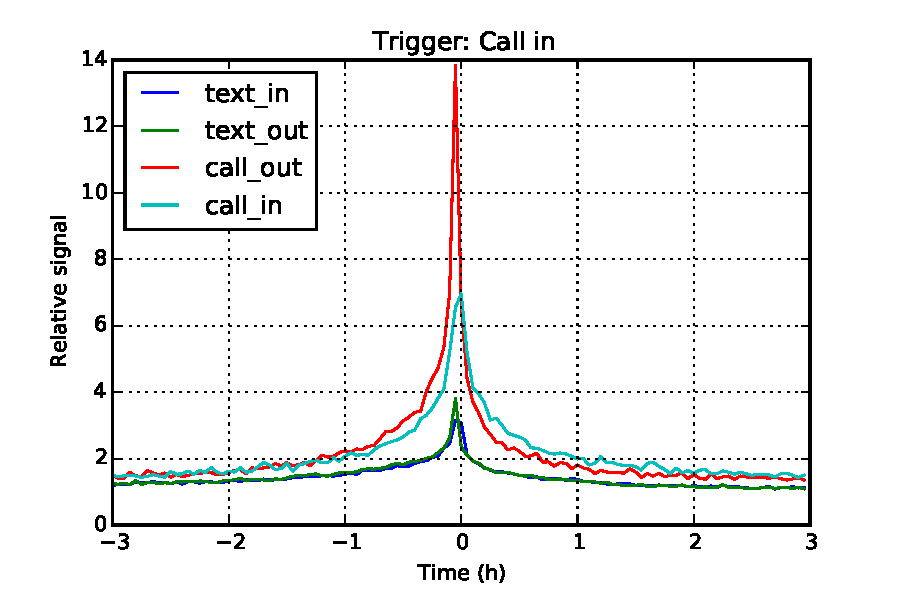
\includegraphics[width=\figwidth, height=\dualheight, keepaspectratio]{pics/dtu/call_in-int10800-bin180.pdf}
	}\\
	\subbottom[Relative activity of events triggered by outgoing calls.]{%
		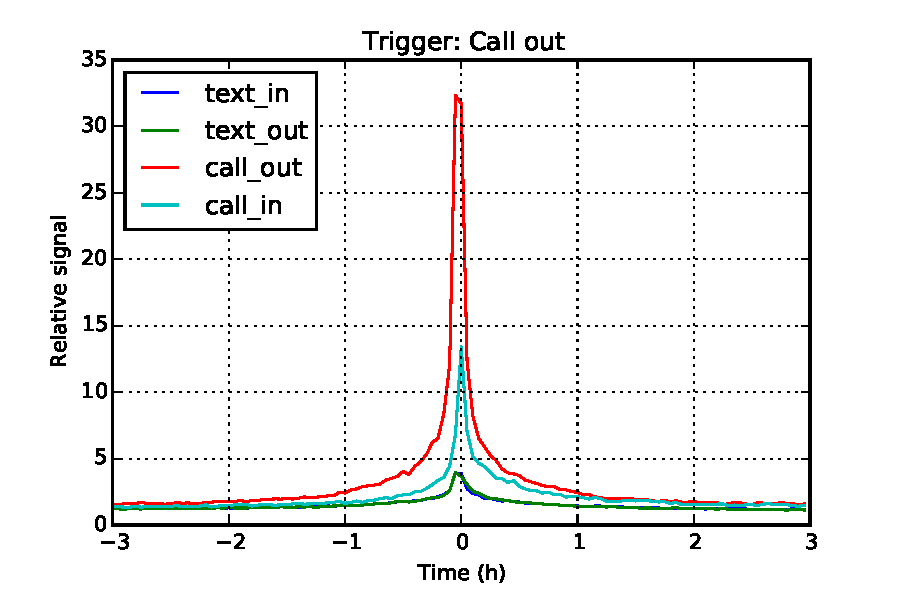
\includegraphics[width=\figwidth, height=\dualheight, keepaspectratio]{pics/dtu/call_out-int10800-bin180.pdf}}
	\caption{Comparison of the increased activity caused by incoming and outgoing calls over an interval of $\pm$ 3 hours around an event with bins of three minutes.}
	\label{fig:calls_three_minutes}
\end{figure}
\begin{figure} %[htb]
	\centering
	\subbottom[Relative activity of events triggered by incoming calls.]{
%		\label{label 1}	
		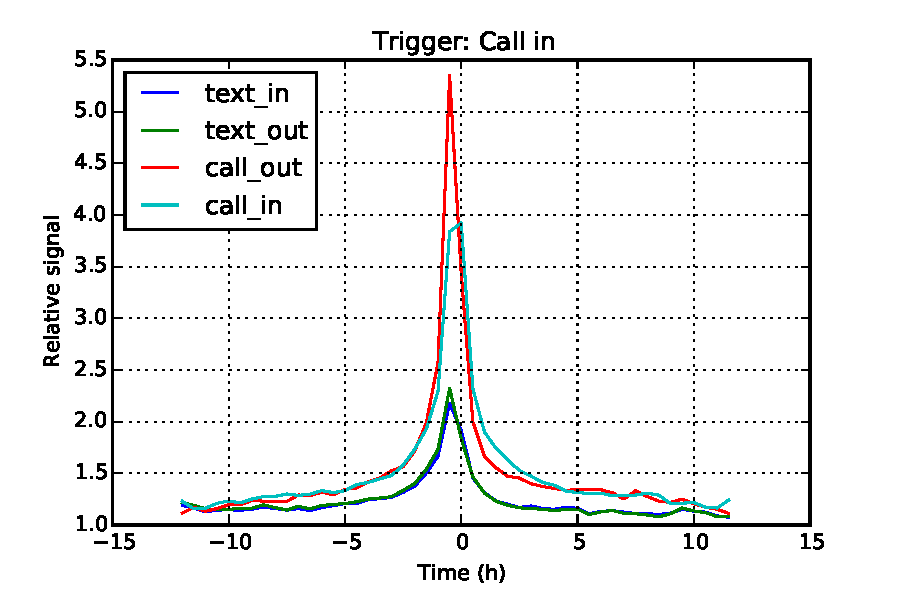
\includegraphics[width=\figwidth, height=\dualheight, keepaspectratio]{pics/dtu/call_in-int43200-bin1800.pdf}
	} \\
	\subbottom[Relative activity of events triggered by outgoing calls.]{
		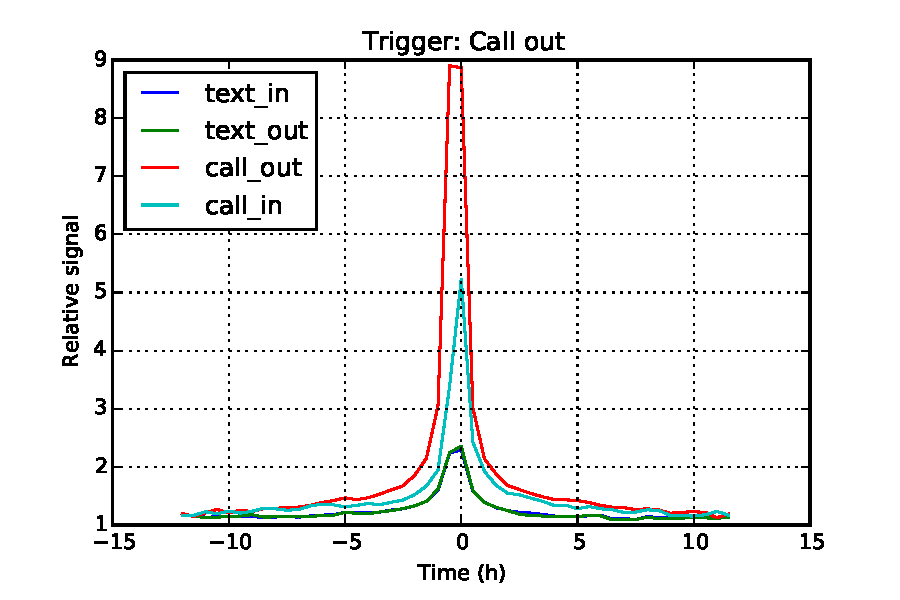
\includegraphics[width=\figwidth, height=\dualheight, keepaspectratio]{pics/dtu/call_out-int43200-bin1800.pdf}
	}
	\caption{Comparison of the increased activity caused by incoming and outgoing calls over an interval of $\pm$ 12 hours around an event with bins of thirty minutes.}
	\label{fig:calls_half_hour}
\end{figure}
As the figures clearly show, the all four activities increase significantly for the average user around incoming and outgoing calls.

\FloatBarrier
\subsection{Influence of GPS activity}
The raw format of the users' GPS logs looks similar to those of the call and text logs:
\begin{snippet}
	{
		"timestamp": 8058876274, 
		"lon": 6.45051654, 
		"user": "0c28e8f4ad9619bca1e5ea4167e10a", 
		"provider": "gps", 
		"lat": 28.20527041, 
		"id": 6429902, 
		"accuracy": 39.4
	}
\end{snippet}
An analysis similar to that of described in section \ref{sec:trigger_phone} was carried out using GPS phone data as triggers. I chose to define a user as being 'active' if they travelled at an average speed of $\unitfrac[0.5]{m}{s}$ between two consecutive GPS log entries, while discarding measurements closely following each other. The reason for this is that the uncertainty on the location measurements could yield false measurements of high average speeds when the measurements are not temporally separated. A lot of the measurements turned out to be grouped somewhat tightly - for instance, approximately $80\%$ of the time intervals were below $\unit[100]{s}$. This occurs because the Social Fabric data not only actively records its users' locations with some set interval, but also passively records the location when another app requests it, so when users spend time on apps that need to continually update their position such as Google Maps, a location log entry is written every second. The distribution of intervals between consecutive GPS measurements is shown in figure \ref{fig:gps_spacings}.
\begin{figure}[htbp]
	\centering
	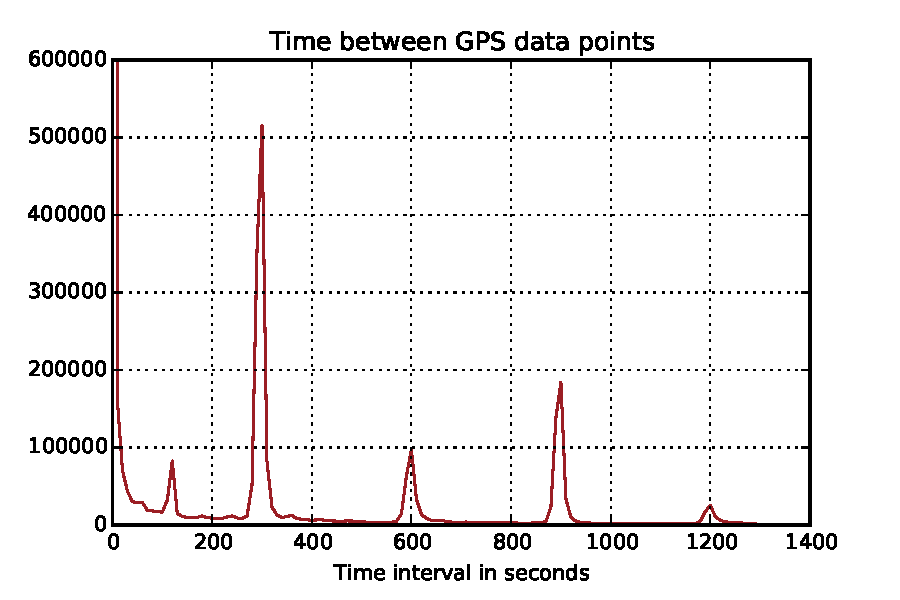
\includegraphics[width = \textwidth]{pics/dtu/gps_spacings.pdf}
	\caption{Plot of typical temporal spacings between consecutive GPS measurements.}
	\label{fig:gps_spacings}
\end{figure}
A typical uncertainty on civilian GPS devices is at most $\unit[100]{m}$\cite{gps_precision}, so because I choose to consider a user active if they travel at a mean speed of $\unitfrac[0.5]{m}{s}$, and based on the time spacings shown in figure \ref{fig:gps_spacings}, I chose to discard measurements separated by less than $\unit[500]{s}$.

An analysis like that of section \ref{sec:trigger_phone} reveals that a user's phone activity is significantly increased around times when they are on the move, as shown in figure \ref{fig:trigger_gps}.
\begin{figure} %[htb]
	\centering	
	\subbottom[Interval: 5 hours. Bin size: 5 minutes.]{
		\label{fig:trigger_gps_short}
		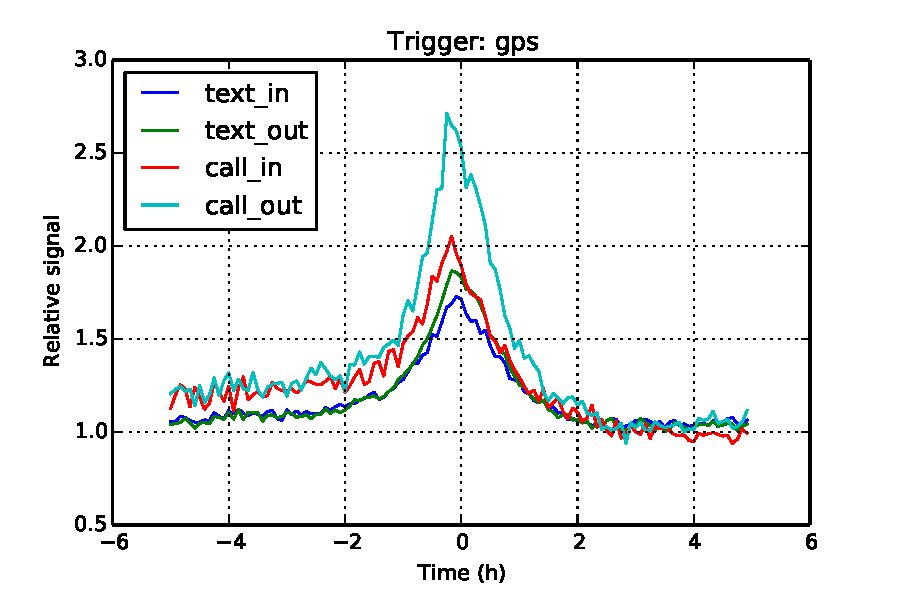
\includegraphics[width=\figwidth, height=\dualheight, keepaspectratio]{pics/dtu/gps-int18000-bin300.pdf}
	} \\
	\subbottom[Interval: 24 hours. Bin size: 15 minutes.]{
		\label{fig:trigger_gps_long}
		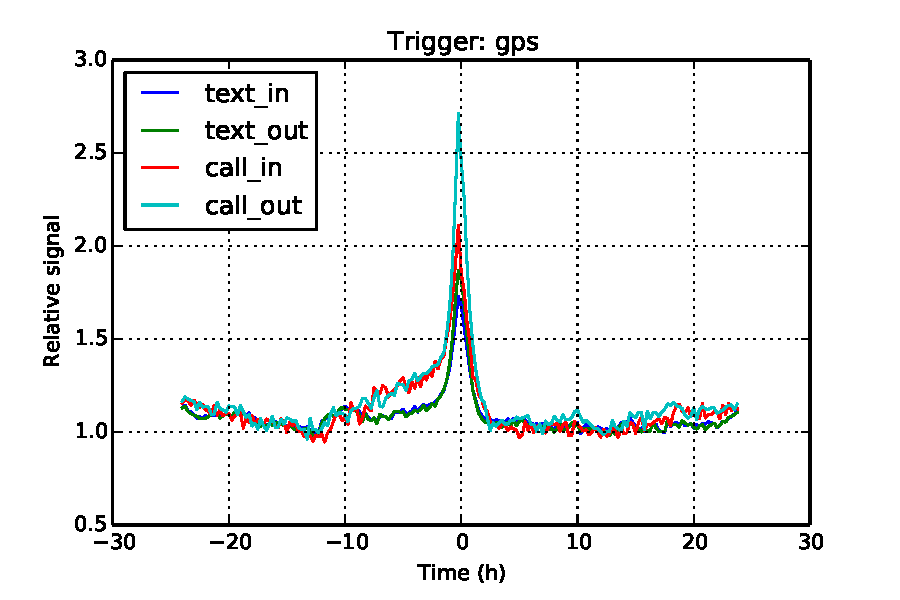
\includegraphics[width=\figwidth, height=\dualheight, keepaspectratio]{pics/dtu/gps-int86400-bin900.pdf}
	}
	\caption{Relative increase of activities triggered by GPS activity.}
	\label{fig:trigger_gps}
\end{figure}
Note the asymmetry of the signal, especially visible in figure \ref{fig:trigger_gps_short}. After a measurement of a user being active, the signal dies off about two and a half hours into the future, whereas it persists much longer into the past. Concretely, this means that people's phone activity (tendency to call or text) becomes uncorrelated with their physical activity after roughly two and a half hours, whereas their tendency to move around is increased for much longer time after calling or texting.

The relative signal in figure \ref{fig:trigger_gps_long} appears to be increasing at around $\pm \unit[24]{h}$, which would seem reasonable assuming people have slightly different  sleep schedules - if a person is on the move and hence more likely to place a call at time $t=0$, they're slightly more likely than the general user to be on the move around $t = \unit[\pm 24]{h}$. Figure \ref{fig:gps_longest} shows the same signal extended to $\unit[\pm 36]{h}$ where slight bumps are visible 24 hours before and after activity.
\begin{figure} %[htb]
	\centering
	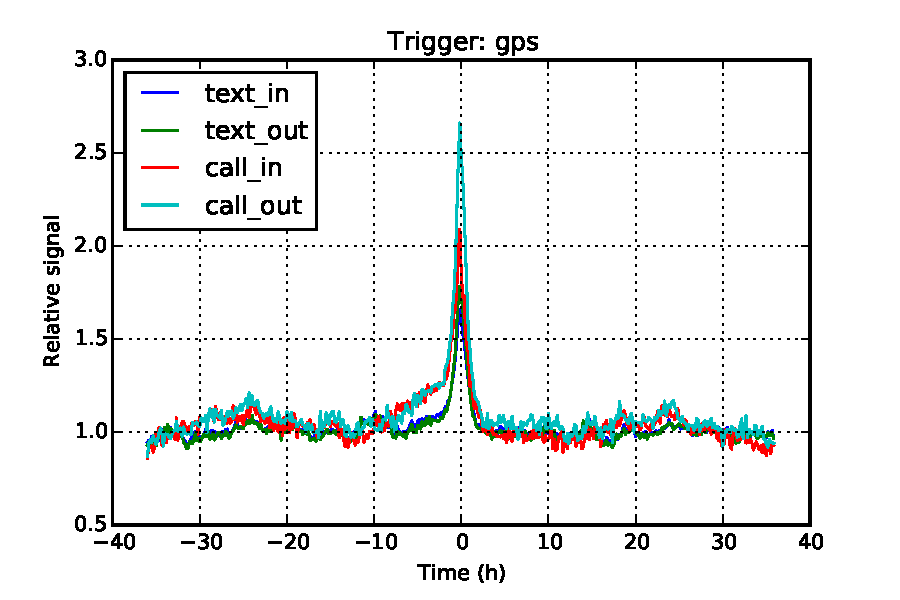
\includegraphics[width=\figwidth]{pics/dtu/gps-int129600-bin600.pdf}
	\caption{GPS-triggered activity increase over an interval of 36 hours using a bin size of 10 minutes.}
	\label{fig:gps_longest}
\end{figure}

\FloatBarrier
\subsection{Influence of Bluetooth signal}
\label{sec:trigger_bluetooth}
The following is a randomized entry in a user's bluetooth log.
\begin{snippet}
	{
		"name": "d5306a3672b7a0b8f9696d294ec4b731", 
		"timestamp": 6870156680, 
		"bt_mac": "1f158ae269d69efa5bb4794ee2a0b2dd68bd3a9badfeaf70f258ad3c74b0c09b", 
		"class": 1317046, 
		"user": "41cdb7ecaaaec3d33391ed063e7fa2", 
		"rssi": -76, 
		"id": 4139043
	}
\end{snippet}
The 'bt\_mac' entry is the MAC-adress of the device which the Bluetooth receiver in the user's phone has registered, so it is reasonable to assume several different MAC addresses occur at several consecutive timestamps. I call the number of repeated MAC adresses needed for a user to be considered social the 'social threshold'. Figures \ref{fig:trigger_bluetooth1}, \ref{fig:trigger_bluetooth2} and \ref{fig:trigger_bluetooth4} show the increased activity around times when users were considered social with a threshold of 1, 2 and 4 repeated pings.
\begin{figure} %[htb]	
	\centering
	\subbottom[Interval: 12 hours, Bin size: 10 minutes.]{
		\label{fig:trigger_bluetooth_short}
		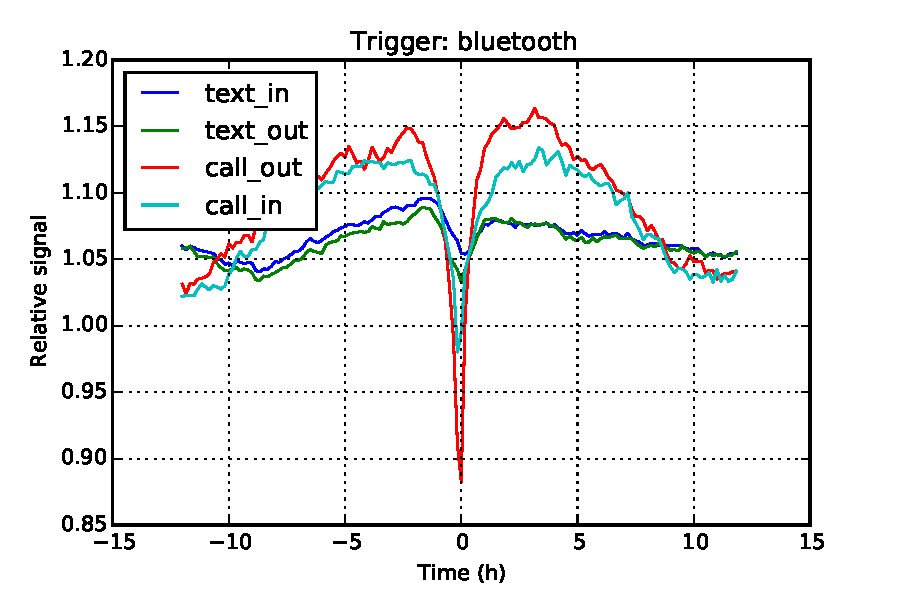
\includegraphics[width=\figwidth, height=\dualheight, keepaspectratio]{pics/dtu/bluetooth_1-int43200-bin600.pdf}
	} \\
	\subbottom[Interval: 36 hours, Bin size: 15 minutes.]{
		%		\label{label 1}
		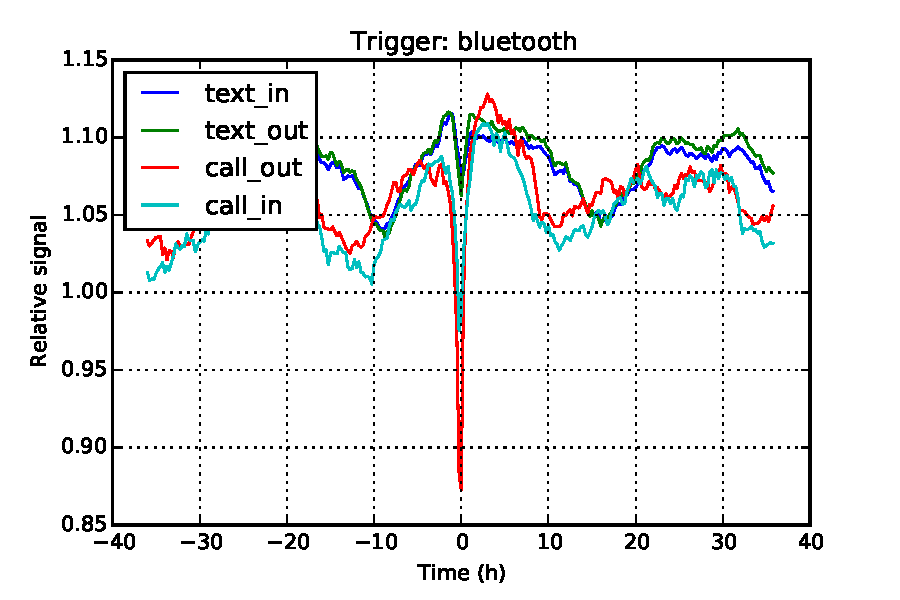
\includegraphics[width=\figwidth, height=\dualheight, keepaspectratio]{pics/dtu/bluetooth_1-int129600-bin900.pdf}
	}
	\caption{The effect on phone activity of sociality as measured by the user's Bluetooth signal. The threshold used for being considered social as one repeated signal.}
	\label{fig:trigger_bluetooth1}
\end{figure}

\begin{figure} %[htb]	
	\centering
	\subbottom[Interval: 12 hours, Bin size: 10 minutes.]{
		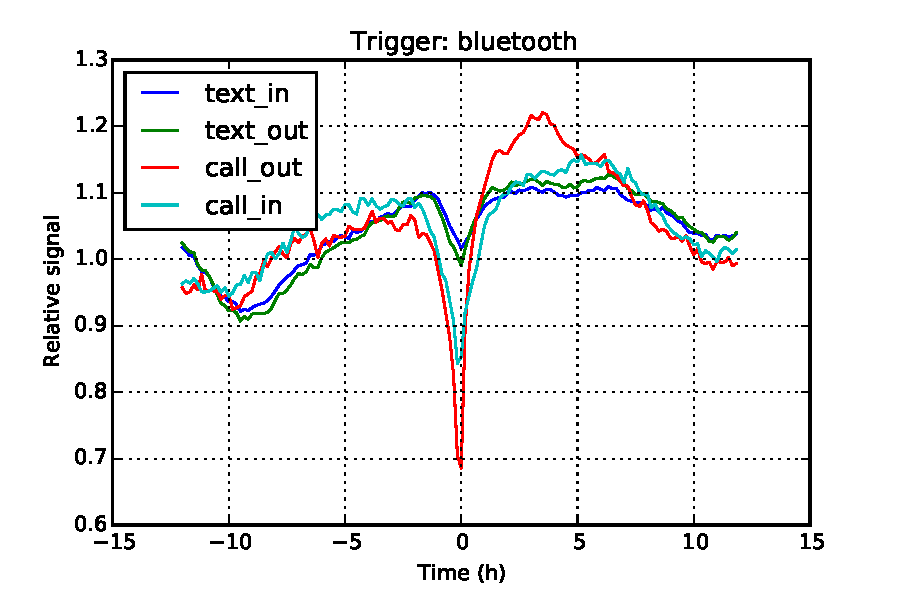
\includegraphics[width=\figwidth, height=\dualheight, keepaspectratio]{pics/dtu/bluetooth_2-int43200-bin600.pdf}
	} \\
	\subbottom[Interval: 36 hours, Bin size: 15 minutes.]{
		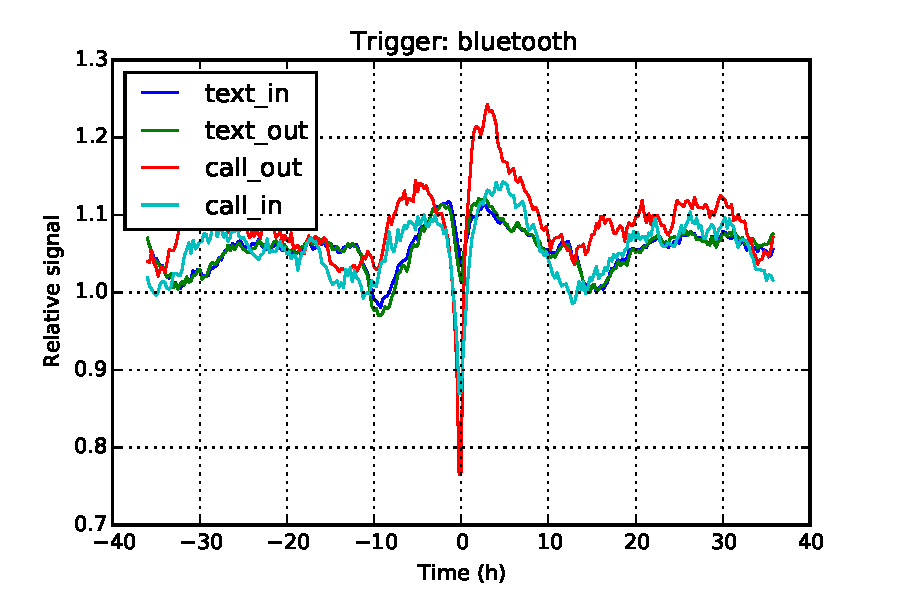
\includegraphics[width=\figwidth, height=\dualheight, keepaspectratio]{pics/dtu/bluetooth_2-int129600-bin900.pdf}
	}
	\caption{The effect on phone activity of sociality as measured by the user's Bluetooth signal. The threshold used for being considered social as two repeated signals.}
	\label{fig:trigger_bluetooth2}
\end{figure}

\begin{figure} %[htb]
	\centering
	\subbottom[Interval: 12 hours, Bin size: 10 minutes.]{
		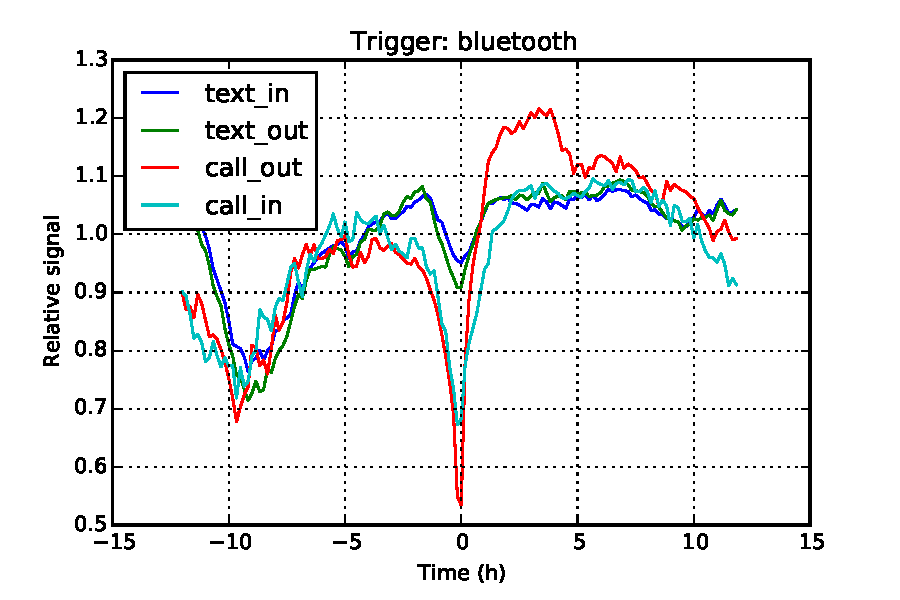
\includegraphics[width=\figwidth, height=\dualheight, keepaspectratio]{pics/dtu/bluetooth_4-int43200-bin600.pdf}
	} \\
	\subbottom[Interval: 36 hours, Bin size: 15 minutes.]{
		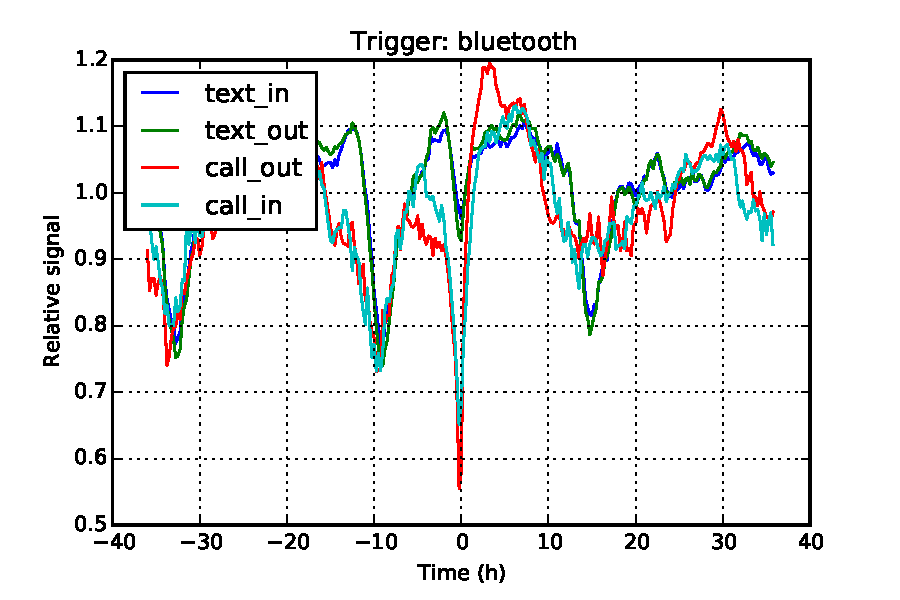
\includegraphics[width=\figwidth, height=\dualheight, keepaspectratio]{pics/dtu/bluetooth_4-int129600-bin900.pdf}
	}
	\caption{The effect on phone activity of sociality as measured by the user's Bluetooth signal. The threshold used for being considered social as four repeated signals.}
	\label{fig:trigger_bluetooth4}
\end{figure}
Contrary to the previous analyses, phone activities decreased somewhat when users were social. As stated, each of these analyses were fairly similar, I've only explicitly included the code used to extract and save Bluetooth data, as well as the code used to load the data and generate figures \ref{fig:trigger_bluetooth1} through \ref{fig:trigger_bluetooth4}. This code is included in section \ref{sec:communication_dymanic_code}.
\section{Extraction of Input Data}
\label{sec:data_extraction}
The predictive powers of mobile phone behaviour on the user's psychological profile is currently an area of \todo{1000 kilder!!!} active research. As part of my thesis work, I have tried to predict the psychological profiles of the SFP participants using various machine learning methods on the available phone logs.

The software I've written first preprocesses the phone logs to extract various relevant parameters, then collects the parameters and psychological profile scores for each user to serve as input and output, respectively, for the various learning methods. Many of the parameters are chosen following a recent article by de Montjoye et al\cite{demontjoye2013}. The following contains an outline and brief explanation of the extracted parameters.

This section contains a list of the extracted parameters used for psychological profiling along with a brief description of the extraction process when necessary. The preprocessing code is included in section \ref{sec:preprocess.py}.

\subsection{Simple Call/Text Data}
The most straightforward data type is the timestamps from a given user's call/text logs. Six of the parameters used were simply the standard deviation and median of the times between events in the logs for each user's call log, text log, and the combination thereof, excluding time gaps of more than three says on the assumption that it would indicate a user being on vacation or otherwise having a period of telephone inactivity. The entropy $S_u$ of each of the three was also included simply by computing the sum
\begin{equation}
	S_u = - \sum_c \frac{n_c}{n_t} \ln_2{\frac{n_c}{n_t}}, \label{eqn:contact_entropy}
\end{equation}
where $c$ denotes a given contact and $n_t$ the total number of interactions, and $n_c$ the number of interactions with the given contact. The number of contacts, i.e. the number of unique phone numbers a given user had contacted by means of calls, texts, and the combination thereof, was also extracted along with the total number of the various kinds of interactions and the contact to interaction ratios. The response rates, defined as the rate of missed calls and incoming texts, respectively, that a given user replied to within an hour, where also determined along with the text latency defined as the median test response time. Finally the percentage calls and texts that were outgoing was determined as well as the fraction of call interactions that took places during the night, defined as between 22-08.

\subsection{Location Data}
A number of parameters based on the spacial dynamics of the user were also extracted. Among these is the radius of gyration, meaning simply the radius of the smallest enclosing circle enclosing all the registered locations of the user on the given day, and the distance travelled per day. I chose to extract the median and standard deviation of each, filtering out the radii that exceeded 500km so as to keep information about long distance travels in the distance parameter and information about travel within a given region in the radius of gyration parameter.

\subsubsection{Cluster Analysis}
One parameter which has strong links\cite{demontjoye2013} to psychological traits is the number of locations in which the user typically spends time, and the entropy of their visits to that location. Hence, the task at hand is to identify dense clusters of GPS coordinates for each user. This is a typical example of a task which is very intuitive and quickly approximated by humans, but is extremely computationally expensive to solve exactly. Concretely, the problem of finding the optimal division of $n$ data points into $K$ clusters is formulated as minimizing the 'score' defined as
\begin{equation}
	S = \sum_K \sum_{x_n \in C_k} |x_n - c_k|^2, \label{eqn:lloyd_minimize}
\end{equation}
where $c_k$ denotes the centroid of the cluster $C_k$. Each point $x_n$ is assigned to the cluster corresponding to the nearest centroid. The usual way of approaching this problem is to use Lloyd's algorithm, which consists of initializing the centroids randomly, assigning each point to the cluster corresponding to the centroid which is nearest, then moving each centroid to the center of its points and repeating the last two steps until convergence. As this isn't guaranteed to converge on the global minimum of \eqref{eqn:lloyd_minimize}, the process can be repeated a number of times, keeping only the result with the lowest value of $S$. I accomplished this by writing a small Python module to perform various variations of Lloyd's algorithm and to produce plots of the resulting clusters. The code is included in section \ref{sec:lloyds.py}.

This allows one to implement Lloyd's algorithm and visualize its result easily, as the code allows automatic plotting of the result from the algorithm while automatically selecting different colors for the various clusters. As an example, the following code snippet generates 1000 random points, runs Lloyd's algorithm to determine clusters and saves a plot of the results.
\begin{snippet}
	points = [[random.uniform(-10,10), random.uniform(-10,10)] for _ in xrange(10**3)]
	clusters = lloyds(X = points, K = 6, runs = 1)
	draw_clusters(clusters = clusters, filename = 'lloyds_example.pdf')
\end{snippet}
This results in the following visualization:
\begin{center}
	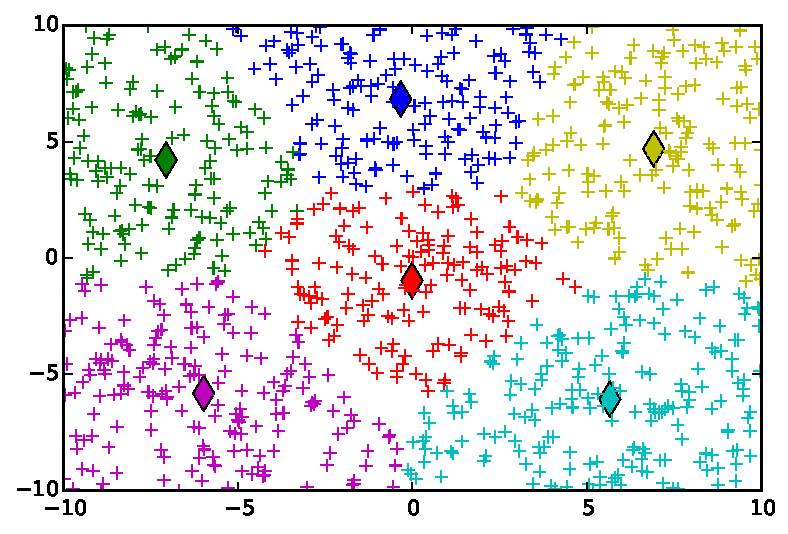
\includegraphics[width=0.45\textwidth]{pics/dtu/lloyds_example.pdf}
\end{center}
I chose to modify the algorithm slightly on the following basis: Usually, the algorithm takes as its initial centroids a random sample of the data. I'll call this 'sample' initialization. This leads to a greater number of clusters being initialized in the areas with an increased density of data points, meaning that centroids will be highly cluttered at first, 'fighting' over the dense regions of data points then slowly spreading out. A few such iterations are shown in figure \ref{fig:lloyds_convergence_sample}.
\begin{figure} %[htbp]
	\centering
	\subbottom[]{
		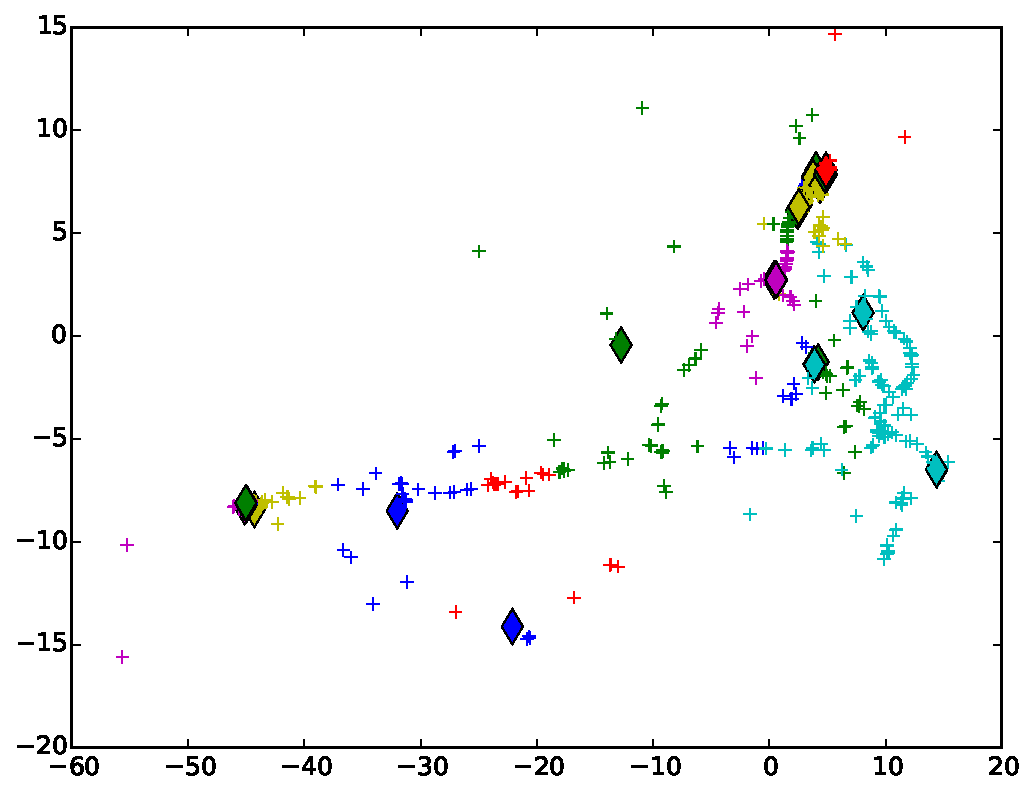
\includegraphics[width=0.45\textwidth, height=\dualheight, keepaspectratio]{pics/dtu/lloyd_con_sample_1.pdf}
	}
	\subbottom[]{
		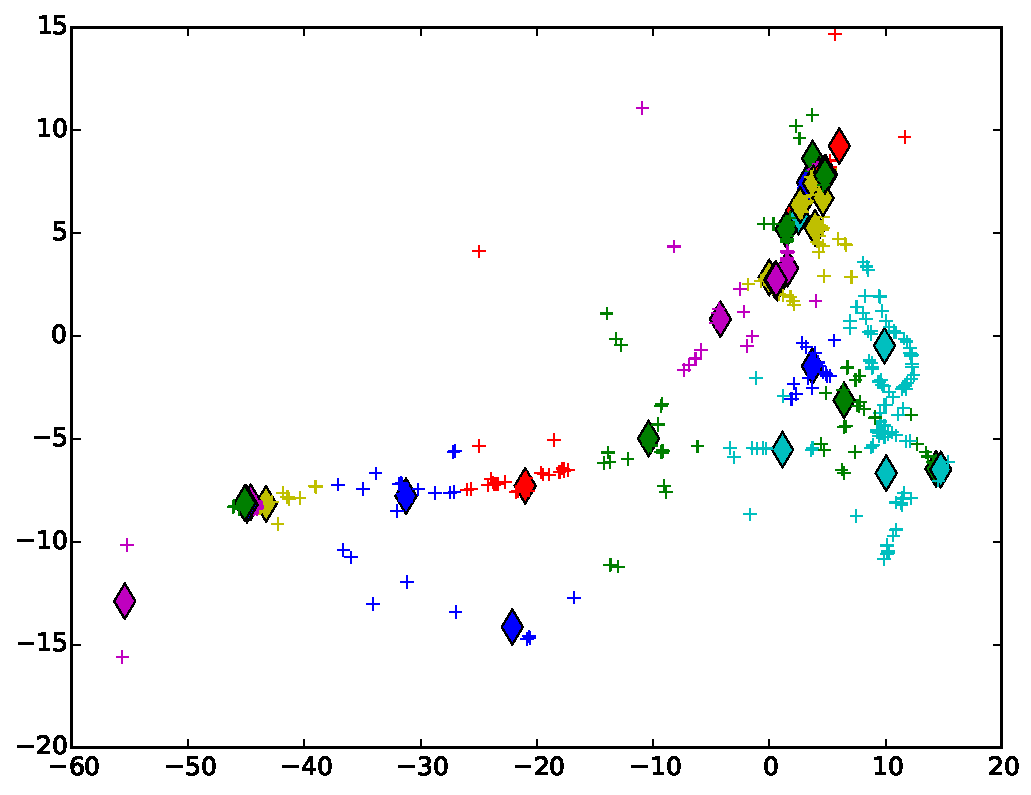
\includegraphics[width=0.45\textwidth, height=\dualheight, keepaspectratio]{pics/dtu/lloyd_con_sample_2.pdf}
	}
	\subbottom[]{
		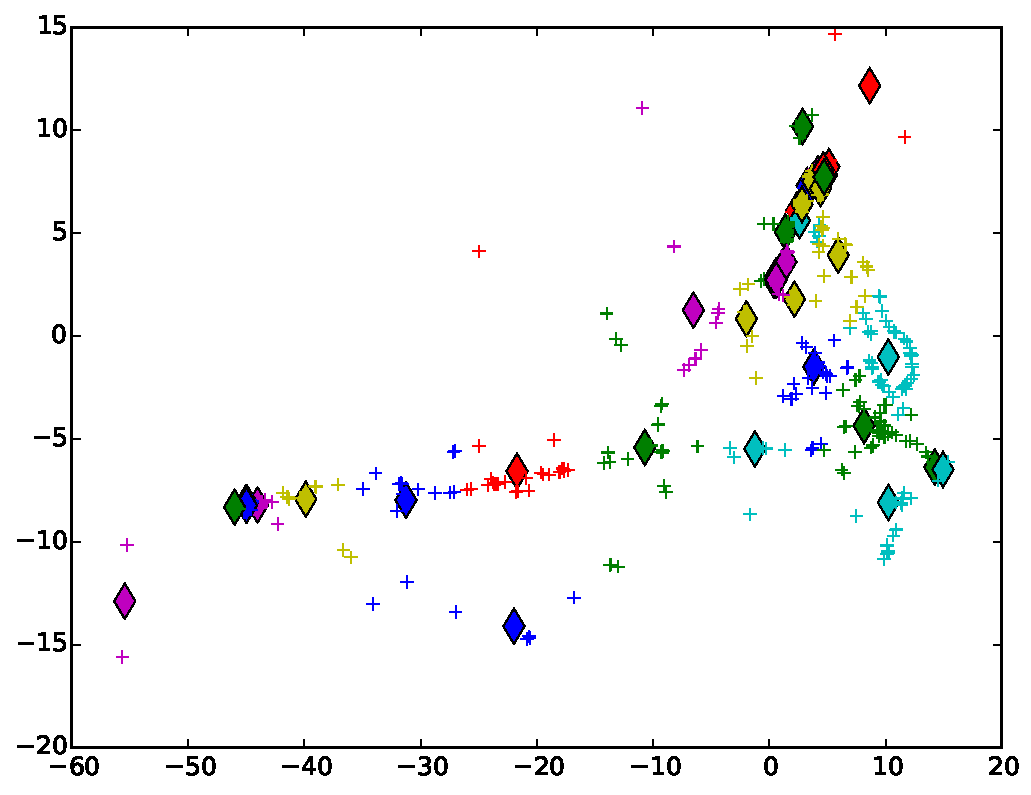
\includegraphics[width=0.45\textwidth, height=\dualheight, keepaspectratio]{pics/dtu/lloyd_con_sample_3.pdf}
	}
	\subbottom[]{
		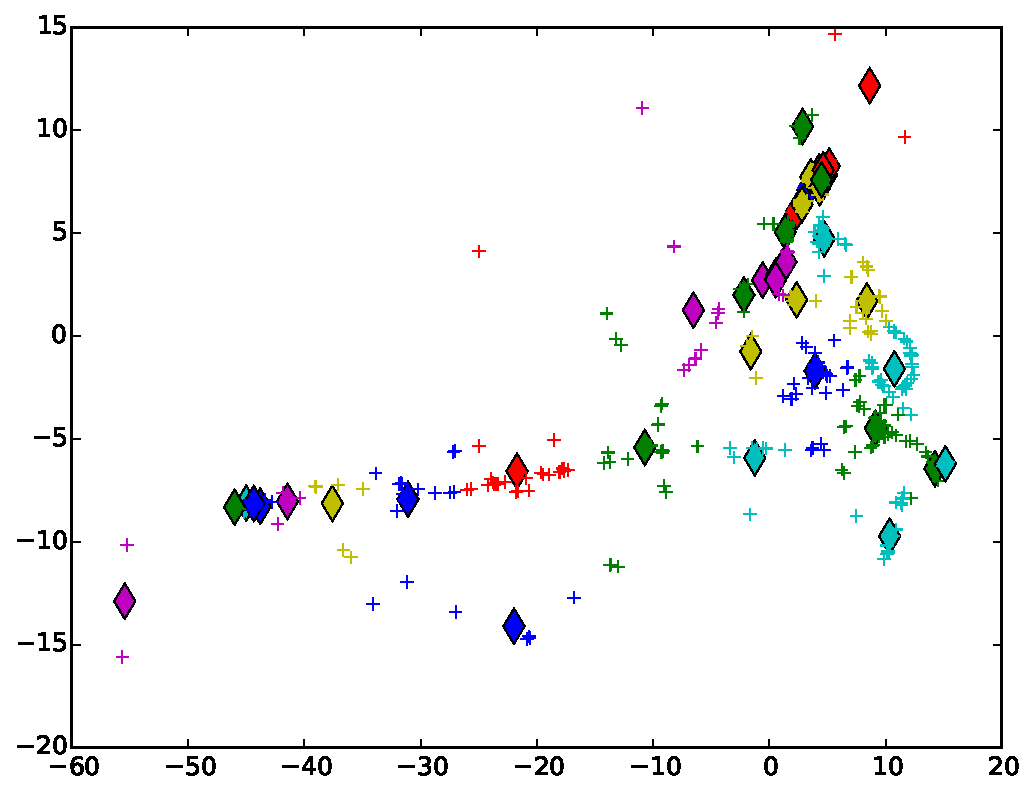
\includegraphics[width=0.45\textwidth, height=\dualheight, keepaspectratio]{pics/dtu/lloyd_con_sample_4.pdf}
	}
	\caption{A few iterations of Lloyd's algorithm using 'sample' initialization. The axes denote the distance in km to some typical location for the user. Note that clusters are initially cluttered, then slowly creep away from the denser regions.}
	\label{fig:lloyds_convergence_sample}
\end{figure}
However, this method is dangerous: The goal is to identify locations in which a user spends much of their time, i.e. in which more than some threshold of their GPS pings originated, and this initialization is likely to 'cut' the more popular locations into several clusters, neither of which contains more data points than the threshold. One example might be the DTU campus, which is a risk of being divided into several locations with too few data points in each, giving the false impression that user doesn't visit the campus that often. To avoid this effect, I implemented another initialization, 'scatter', in which the clusters start out on points select randomly from the entire range of $x,y$-values in the user's dataset. This turned out to not only solve the problem described above, but also converge much quicker and reach a slightly lower score as define in \eqref{eqn:lloyd_minimize}. A few such iterations are shown in figure \ref{fig:lloyds_convergence_scatter}.
\begin{figure} %[htb]
	\centering
	\subbottom[]{
		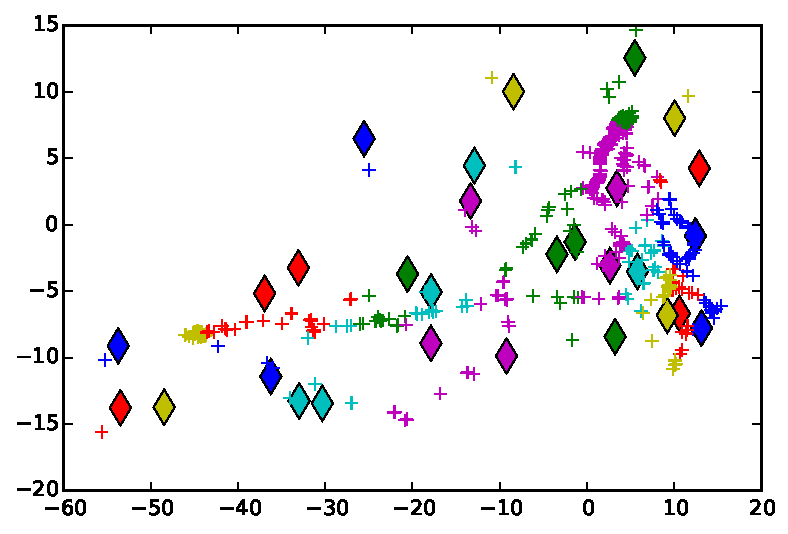
\includegraphics[width=0.45\textwidth, height=\dualheight, keepaspectratio]{pics/dtu/lloyd_con_scatter_1.pdf}
	}
	\subbottom[]{
		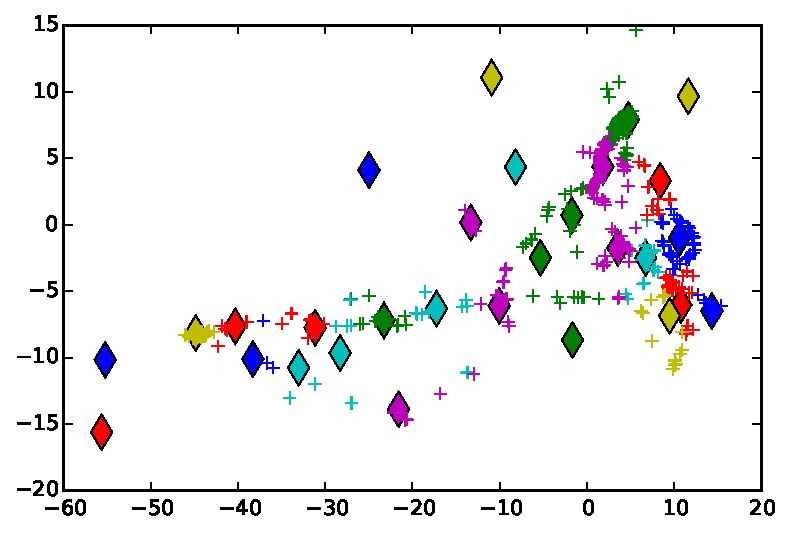
\includegraphics[width=0.45\textwidth, height=\dualheight, keepaspectratio]{pics/dtu/lloyd_con_scatter_2.pdf}
	}
	\subbottom[]{
		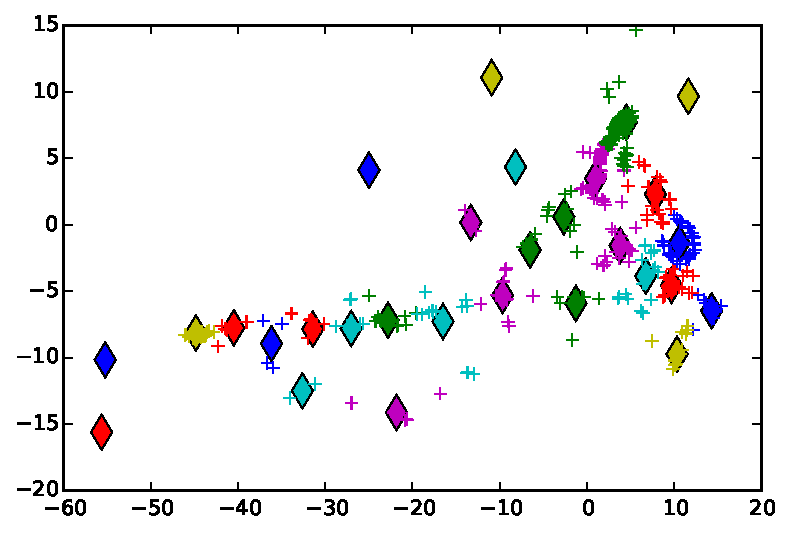
\includegraphics[width=0.45\textwidth, height=\dualheight, keepaspectratio]{pics/dtu/lloyd_con_scatter_3.pdf}
	}
	\subbottom[]{
		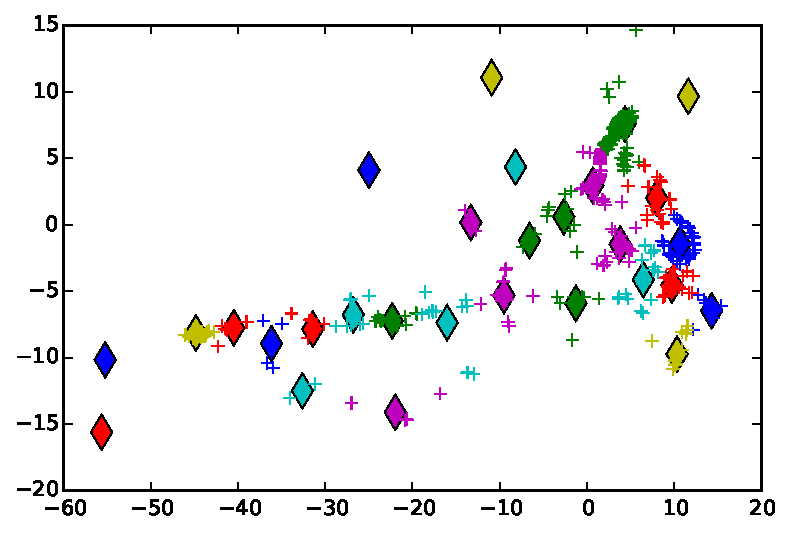
\includegraphics[width=0.45\textwidth, height=\dualheight, keepaspectratio]{pics/dtu/lloyd_con_scatter_4.pdf}
	}
	\caption{A few iterations of Lloyd's algorithm using 'scatter' initialization. The axes denote the distance in km to some typical location for the user. Note that clusters are initially randomly spread across the entire range of $x,y$-values and converge quickly to a local minimum for \eqref{eqn:lloyd_minimize}.}
	\label{fig:lloyds_convergence_scatter}
\end{figure}
The difference in end results for the two methods is exemplified in figure \ref{fig:lloyds_result_comparison}.
\begin{figure} %[htbp]
	\centering
	\subbottom[Sample initialization.]{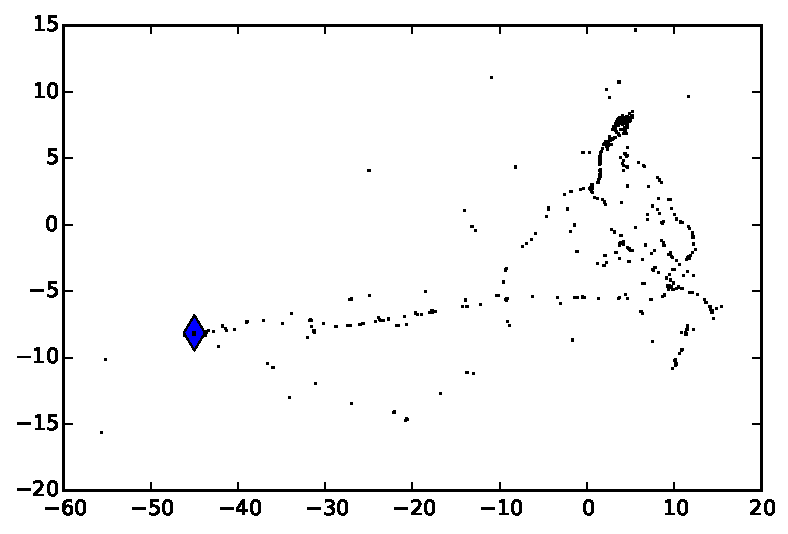
\includegraphics[height=\dualheight]{pics/dtu/final_sample_100_5.pdf}}
	\subbottom[Scattered initialization.]{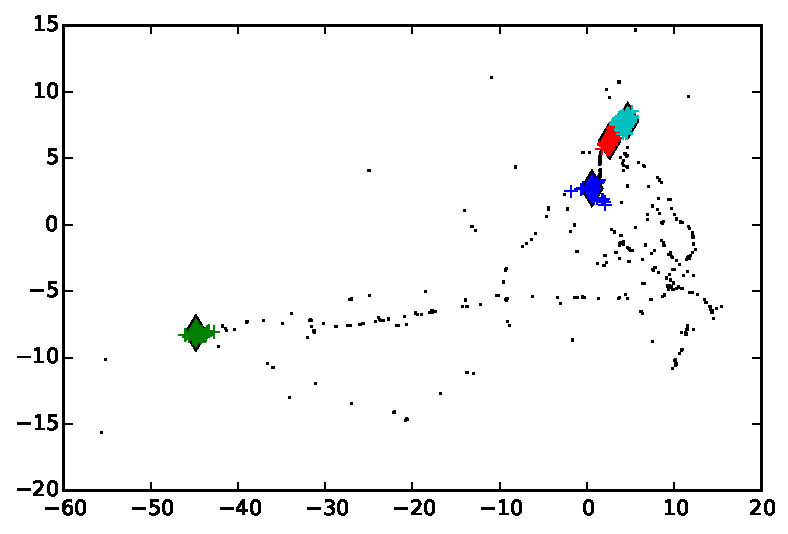
\includegraphics[height=\dualheight]{pics/dtu/final_scatter_100_5.pdf}}
	\caption{Comparison of the final results of the two initialization methods using 100 initial clusters, a threshold of $5\%$ of the data points before a cluster is considered a popular location and running the algorithm 10 times and keeping the best result. Clusters containing more than $5\%$ of the total amount of data points are in color, whereas the remaining points are black dots.}
	\label{fig:lloyds_result_comparison}
\end{figure}
While this works great for users who stay in or around Copenhagen, it will cause problems for people who travel a lot. A user who has visited Australia, for instance, will have their initial clusters spread out across the globe, and it's highly likely that one them will end up representing all of Denmark. I ended up simply running both versions and keeping the result yielding the highest amount of locations.

\FloatBarrier
\subsection{Time Series Analysis}
\label{sec:ar}
Another interesting aspect to include is what one somewhat qualitatively might call behavioural regularity - some measure of the degree in which a user's phone activities follow a regular pattern. Quantifying this turns out to take a bit of work. First of all, any user's activity would be expected to closely follow the time of day, so the timestamps of each user's outgoing texts and calls are first converted into 'clock times' meaning simply the time a regular clock in Copenhagen's time zone would display at the given time. This process is fairly painless when using e.g. the UTC time standard, which does not observe daylight saving time (DST), but some subtleties arise in countries that do use DST, as this makes the map from Unix/epoch time to clock time 'almost bijective' - when changing \emph{away} from DST, two consecutive hours of unix time map to the same clock time period (02:00 to 03:00), whereas that same clock period is skipped when changing \emph{to} DST. The most commonly used Python libraries for datetime arithmetic accommodate this by including a dst boolean in their datetime objects when ambiguity might arise, however I simply mapped the timestamps to clock times and ignored the fact twice a year, one time bin will artificially contain contributions from one hour too many or few. One resulting histogram is shown in figure \ref{fig:ar_histogram_raw}. \todo{Tilføj lidt om AR-serier når du har bogen!!!} %og tilføj den til refs!!!
\begin{figure}
	\centering
	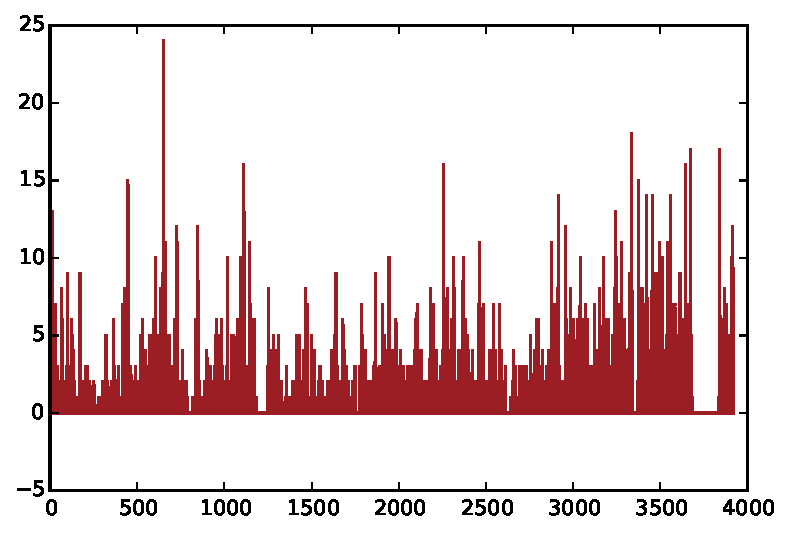
\includegraphics[width = \figwidth]{pics/dtu/ar_signal_example.pdf}
	\caption{Histogram of a user's outgoing calls and texts with a bin size of six hours.}
	\label{fig:ar_histogram_raw}
\end{figure}

\subsection{Facebook Data}
Unfortunately, the only available Facebook data was a list of each user's friends, so the only contribution of each user's Facebook log was the number of friends the user had.

\subsection{Bluetooth Data}
I extracted a number of different features from each user's Bluetooth log file. First, I set a threshold for when a given user is considered social, as described in section \ref{sec:trigger_bluetooth}. I chose to use a threshold of two. I then tried to estimate how much time each user spends in the physical company of others in the following way: for each time stamp in the user's Bluetooth log, I checked if the user was social or not and assumed that this status was the same until the following log entry, unless the delay was more than two hours. The rationale behind this is to avoid skewing the measurements if a user turns off their phone for extended periods of time. Otherwise, e.g. studying with a few friends at DTU, turning off your phone and going on vacation for two weeks would give the false impression that the user were highly social for a long period of time. I then recorded the fraction of times the user was estimated as being social in this fashion.

Finally, I also wanted some measure of the degrees to which a user's social behaviour follows a pattern. I looked for temporal patterns by fitting AR-series and computing autocorrelation coefficients for each user's social behaviour as described in section \ref{sec:ar}. I also chose to compute a 'social entropy' much like \eqref{eqn:contact_entropy}, but weighted by the time the user spends with each acquaintance:
\begin{align}
	E &= -\sum_i f_i \ln_2\pp{f_i}, \\
	f_i &= \frac{\text{time spent with $i$}}{\sum_j\text{time spent with $j$}}. \label{eqn:grimbroekmedtekstoverdethele}
\end{align}
Note that the denominator of \eqref{eqn:grimbroekmedtekstoverdethele} is not equal to the total amount of time spent being social, as the contribution from each log entry is multiplied by the number of people present.

\section{Output Data}
\label{sec:output_data}
The main emphasis of this part of the thesis is on predicting so-called \textit{Big Five} personality traits. This section contains a brief description of those, following\cite{Digman1990}.
\textbf{Extraversion} signifies how extroverted and sociable a person is. People with high extraversion scores are supposed to be more eager to seek the company of others. \textbf{Agreeableness} is supposed to be a measure of how sympathetic or cooperative a person is, whereas \textbf{conscientiousness} denotes constraint, self discipline, level of organization etc.. \textbf{Neuroticism} signify the tendency to experience mood swings, and is complementary to emotional stability. Finally, \textbf{Openness}, also called 'openness to experience', or 'inquiring intellect' in earlier works, signifies thoughtfulness, imagination and so on. These five are collectively referred to as the 'big five' or 'OCEAN' after their initials.

I addition to the above, I also had access to a range self-explanatory traits about the participants such as their gender, whether they smoke etc.

\section[Linear Discriminant Analysis]{Linear Discriminant Analysis \& Gender Prediction}
\label{sec:LDA}
Linear discriminant analysis is basically a dimensionality reduction technique developed by Fisher in 1936 \cite{fisher_original} for separating data points into two or more classes. The general idea is to project a collection of data points in $n$-dimensional variable space, onto the line or hyperplane which maximizes the separation between classes. Representing data points in $n$-space by vectors denoted $x$, the objective is to find a vector $\omega$ such that separation between the projected data points on it
\begin{align}
	y = \omega^T x
\end{align}
is maximized.

To break down the derivation of this method, I will first define a convenient distance measure used to optimize the separation between classes, then solve the resulting optimization problem. For clarity, I'll only describe the case of projection of two classes onto one dimension (i.e. using 'line' rather than 'hyperplane' and so on), although the method generalizes easily.

\subsection{A measure of separation for projected Gaussians}
If the projected data points for two classes $a$ and $b$ follow distributions $\mathcal{N}_a$ and $\mathcal{N}_b$, which are standard Gaussians, $\mathcal{N}_i(x) = \mathcal{N}(x;\mu_i, \sigma_i^2)$, the joint probability distribution for the distance between the projections will be the convolution
\begin{align}
	P(x) &= \int_{-\infty}^\infty \mathcal{N}_a(y)\cdot\mathcal{N}_b(x-y) \ud y.
\end{align}
Computing this for a Gaussian distribution,
\begin{align}
	\mathcal{N}(x;\mu, \sigma^2) &= \frac{1}{\sqrt{2\pi}\sigma}e^{-\frac{(x-\mu)^2}{2\sigma^2}},
\end{align}
becomes easier with the convolution theorem, which I'll derive in the following.

Denoting convolution by $*$ and Fourier transforms by
\begin{align}
	\mathcal{F}(f) &= \fnorm \rint f(x)\cdot e^{-i\omega x} \ud x, \label{eqn:fysikerfourier}
\end{align}
the convolution theorem is derived as follows:
\begin{align}
	\mathcal{F}(f*g) &= \fnorm \rint  \rint f(y)\cdot g(x-y) \ud y \, e^{-i\omega x}      \ud \omega, \\
	&= \fnorm \rint f(y) \rint g(x-y) e^{-i\omega x} \ud y \ud\omega, \\
	&= \fnorm \rint f(y) \rint g(z) e^{-i\omega (z+y)} \ud z \ud\omega, \\
	&= \fnorm \rint f(y) e^{-i\omega y} \rint g(z) e^{-i\omega z} \ud z \ud\omega, \\
	\Aboxed{\mathcal{F}(f*g) &= (2\pi)^{n/2} \mathcal{F}(f)\cdot \mathcal{F}(g),} \label{eqn:convolution_theorem}
\end{align}
where the factor in front of the usual form of the theorem $\mathcal{F}(f*g) = \mathcal{F}(f)\cdot \mathcal{F}(g)$ stems from the convention of using angular frequency in Fourier transforms, as in \eqref{eqn:fysikerfourier}, rather than
\begin{align}
	\mathcal{F}(f) &= \rint f(x)\cdot e^{-2\pi i \nu x} \ud x.
\end{align}
Using this, the convolution of two Gaussians can be calculated as
\begin{align}
	\mathcal{N}_a*\mathcal{N}_b &= (2\pi)^{n/2} \mathcal{F}^{-1} \pp{\mathcal{F}(\mathcal{N}_a)\cdot \mathcal{F}(\mathcal{N}_b)}.
\end{align}
The required Fourier transform can be massaged into a nicer form by displacing the coordinate system and cancelling out terms with odd parity:
\begin{align}
	\mathcal{F}(\mathcal{N}(x)) &= \onenorm \infint \frac{1}{\sqrt{2\pi}\sigma} e^{-\frac{(x-\mu)^2}{2\sigma^2}}\cdot e^{-i\omega x} \ud x, \nonumber \\
	&= \frac{1}{2\pi\sigma} \infint e^{-\frac{x^2}{2\sigma^2}} e^{-i\omega(x+\mu)} \ud x, \nonumber \\
	&= \frac{1}{2\pi\sigma}e^{-i\omega\mu} \infint e^{-\frac{x^2}{2\sigma^2}} \pp{\cos(\omega x) + i\sin(\omega x)} \ud x, \nonumber \\
	&= \underbrace{ \frac{1}{2\pi\sigma}e^{-i\omega\mu} }_a \underbrace{\infint e^{-\frac{x^2}{2\sigma^2}} \cos(\omega x)\ud x}_{I(\omega)}. \label{eqn:feynmanstuffgoeshere}
\end{align}
Noting that $I(\omega)$ reduces to an ordinary Gaussian integral at $\omega = 0$ so $I(0) = \sqrt{2\pi}\sigma$, this can be solved with a cute application of Feynman's trick:
\begin{align*}
	\pardiff{I}{\omega} &= - \infint x e^{-\frac{x^2}{2\sigma^2}}\sin(\omega x) \ud x, \\
	&= \infint \sigma^2 \pardiff{}{x}\pp{e^{-\frac{x^2}{2\sigma^2}}}\sin(\omega x) \ud x, \\
	&= \left. \sigma^2 e^{-\frac{x^2}{2\sigma^2}} \sin(\omega x) \right|_{-\infty}^\infty - \omega\infint \sigma^2 e^{-\frac{x^2}{2\sigma^2}}\cos(\omega x) \ud x, \\
	&= -\omega\sigma^2 I(\omega) \Leftrightarrow \\
	I(\omega)&= C e^{-\sigma^2\omega^2/2}, \\
	I(0) = C &= \sqrt{2\pi}\sigma, \\
	I(\omega) &= \sqrt{2\pi}\sigma e^{-\sigma^2\omega^2/2}.
\end{align*}	
Plugging this into \eqref{eqn:feynmanstuffgoeshere} gives the result
\begin{align}
	\mathcal{F}(\mathcal{N}) &= \frac{1}{\sqrt{2\pi}}e^{-i\omega\mu}e^{-\sigma^2\omega^2/2}.
\end{align}
This can be used in conjunction with \eqref{eqn:convolution_theorem} to obtain
\begin{align}
	\mathcal{F}(\mathcal{N}_a*\mathcal{N}_b) &= \sqrt{2\pi} \frac{1}{\sqrt{2\pi}}e^{-i\omega\mu_a}e^{-\sigma_a^2\omega^2/2}\cdot \frac{1}{\sqrt{2\pi}} e^{-i\omega\mu_b}e^{-\sigma_b^2\omega^2/2}, \\
	&= \frac{1}{\sqrt{2\pi}}e^{-i\omega(\mu_a-\mu_b)}e^{-(\sigma_a^2+\sigma_b^2)\omega^2/2},
\end{align}
which is recognized as the transform of another Gaussian describing the separation with $\mu_s = \mu_a - \mu_b$ and ${\sigma_s^2 = \sigma_a^2 + \sigma_b^2}$, so taking the inverse Fourier transformation gives the convolution
\begin{equation}
	\mathcal{N}_a * \mathcal{N}_b = \frac{1}{\sqrt{2\pi}\sigma_s} e^{-\frac{(x-\mu_s)^2}{2\sigma_s^2}}.
\end{equation}
Hence, a reasonable measure of the separation of two projected distributions is
\begin{equation}
	d = \frac{\pp{\mu_a - \mu_b}^2}{\sigma_a^2 + \sigma_b^2}. \label{eqn:broeksomskalmaximeres}
\end{equation}

\subsection{Optimizing separation}
To maximize the separation, the numerator and denominator, respectively, of \eqref{eqn:broeksomskalmaximeres} can be rewritten in terms of $w$ in the following way (using $\widetilde{\mu}_i$ to denote projected means) and simplified by introducing scattering matrices:
\begin{align}
	\pp{\widetilde{\mu}_a - \widetilde{\mu}_b}^2 &= \pp{w^T \pp{\mu_a - \mu_b}}^2, \\
	&= w^T \pp{\mu_a - \mu_b} \pp{\mu_a - \mu_b}^T w, \\
	&= w^T S_B w,
\end{align}
and
\begin{align}
	\widetilde{\sigma}_i^2 &= \sum_{y \in i} \frac{1}{N} \pp{y - \widetilde{\mu}_i}^2, \\
	&= w^T \sum_{y \in i} \pp{x - \mu_i} \pp{x - \mu_i}^T w, \\
	&= w^T S_i w, \\
	\widetilde{\sigma}_a^2 + \widetilde{\sigma}_b^2 &= w^T S_W w,
\end{align}
having introduced the between-class and within-class scatter matrices $S_B$ and $S_W$ by
\begin{align}
	S_B &= \pp{\mu_a - \mu_b} \pp{\mu_a - \mu_b}^T, \\
	S_i &= \sum_{y \in i} \pp{x - \mu_i} \pp{x - \mu_i}^T, \\
	S_W &= S_a + S_b.
\end{align}
Hence, the objective is to solve
\begin{align}
	\frac{\ud }{\ud w} J(w) = \frac{\ud}{\ud w} \pp{ \frac{w^T S_B w}{w^T S_W w} } &= 0, \\
	\frac{ \diff{\,\sqb{w^T S_B w}}{w} w^T S_W w - w^T S_B w \diff{\,\sqb{w^T S_W w}}{w}}{\pp{ w^T S_W w }^2} &= 0, \\
	2 S_B w \cdot w^T S_W w - w^T S_B w \cdot 2 S_W w &= 0, \\
	S_B w - \frac{ w^T S_B w \cdot S_W w}{ w^T S_W w} &= 0, \\
	S_B w - S_W w J(w) &= 0, \\
	S_B w &= S_W w J(w), \\
	S_W^{-1} S_B w &= J(w) w.
\end{align}
The optimal projection vector $w^*$ which satisfies this is \todo{Vær lige sikker på at du forstår det her.}
\begin{equation}
w^* = S_W^{-1}\pp{\mu_a - \mu_b}. \label{eqn:fisher_line}
\end{equation}
Figure \ref{fig:fisher_example} shows a visualization of this that I generated by drawing $(x,y)$ points from two random distributions to simulate two distinct classes of points. If the distributions are independent and Gaussian, the projections will also form Gaussian distributions, and the probability of a new point belonging to e.g. class $a$ given its coordinates $d$ can be estimated using Bayesian probability
\begin{equation}
	P(a|d) = \frac{P(d|a)P(a)}{P(d|a)p(a)+P(d|b)P(b)}, \label{eqn:fisher_class_prob}
\end{equation}
where $P(a)$ and $P(b)$ are simply the prior probabilities for encountering the respective classes, and the conditional probabilities, e.g. $P(d|a)$ are simply given by the value of the projected Gaussian $\mathcal{N}(x';\widetilde{\mu}_a, \widetilde{\sigma}_a)$ at the projected coordinate $x'$. In practise, even when the points are not independent or Gaussian, so that \eqref{eqn:fisher_class_prob} is not a precise estimate of the probability of the point representing a given class, the class with the highest posteriori according to \eqref{eqn:fisher_class_prob} still often turns out to be a good guess.

\begin{figure}
	\centering
	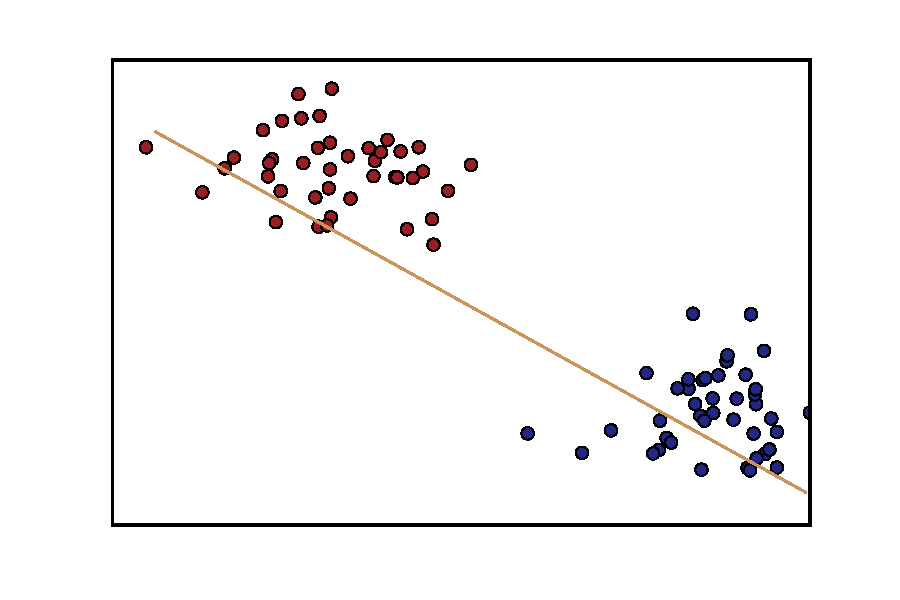
\includegraphics[width = \figwidth]{pics/ml/fisher_example.pdf}
	\caption{Two collections of points drawn from independent Gaussian distributions, representing {\color{moerkeroed} class a} and {\color{oldhat} class b}. If the points are projected onto the {\color{nude} straight line}, which is given by \eqref{eqn:fisher_line}, the separation between the peaks representing the two classes is maximized.}
	\label{fig:fisher_example}
\end{figure}

This method accurately predicted the gender of $79.8\%$ of the participants, which is not particularly impressive as $77.3\%$ of participants were male, so a classifier that assumes that every participant is male would have a comparable success rate. An immediate source of concern is the assumption of linearity: It is possible that the data is ordered in such a way that it is possible to separate data points fairly well based on gender or some psychological trait, just not using a linear classifier. As an extreme example of this, figure \ref{fig:island_example} shows a situation where the points representing one class are grouped together in an 'island' in the middle, isolating them from points representing the remaining class.
\begin{figure}
	\centering
	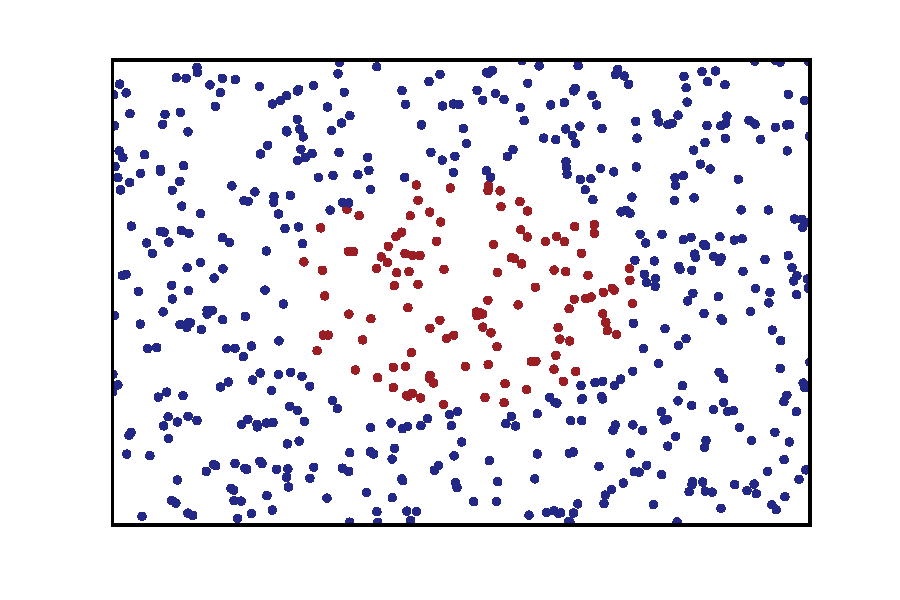
\includegraphics[width = \figwidth]{pics/ml/island_example.pdf}
	\caption{An example of data points representing {\color{moerkeroed} class a} are clearly discernible from those of {\color{oldhat} class b}, yet a linear Fisher classifier fails to predict the classes more precisely than the ratio of {\color{oldhat} b} to {\color{moerkeroed} a}.}
	\label{fig:island_example}
\end{figure}
While it is clear that there's a pattern here, a linear classifier fails to predict classes more precisely than their ratio. Support Vector Machines, or SVMs are another linear classification technique which can be generalized to detect patterns like that in figure~\ref{fig:island_example}. This is described in section \ref{sec:svm}

\chapter[Psychological Profiling]{Psychological Profiling \& Machine Learning}
\label{sec:profiling}
\initial{M}{achine} learning is currently a strong candidate for prediction of psychological profiles from phone data\todo{1000 kilder!!!}. This chapter describes the application of the quantitative data described in setion \ref{sec:data_extraction} and various machine learning schemes, starting with support vector machines (SVMs). \todo{Uddyb når der er flere modeller.}

\section[SVM]{Support Vector Machines}
\label{sec:svm}
The purpose of this section is to introduce SVMs and attempt to apply them to the data obtained in \ref{sec:data_extraction}. The introduction is mainly based on introductory texts by Marti Hearst \cite{hearst1998} and Christopher Burges \cite{burges1998}.
SVMs in their simplest form (\textit{simplest} meaning using a linear kernel, which I'll explain shortly) can be thought of as a slight variation on the linear classifier described in section \ref{sec:LDA}. However, where LDA finds a line such that the distribution of the points representing various classes projected onto the line is maximized, the aim of SVMs is to establish the hyperplane that represents the best possible slicing of the feature space into regions containing only points corresponding to the different classes. A simple example of this is shown in figure \ref{fig:separating_plane_example1}.
\begin{figure}
	\centering
	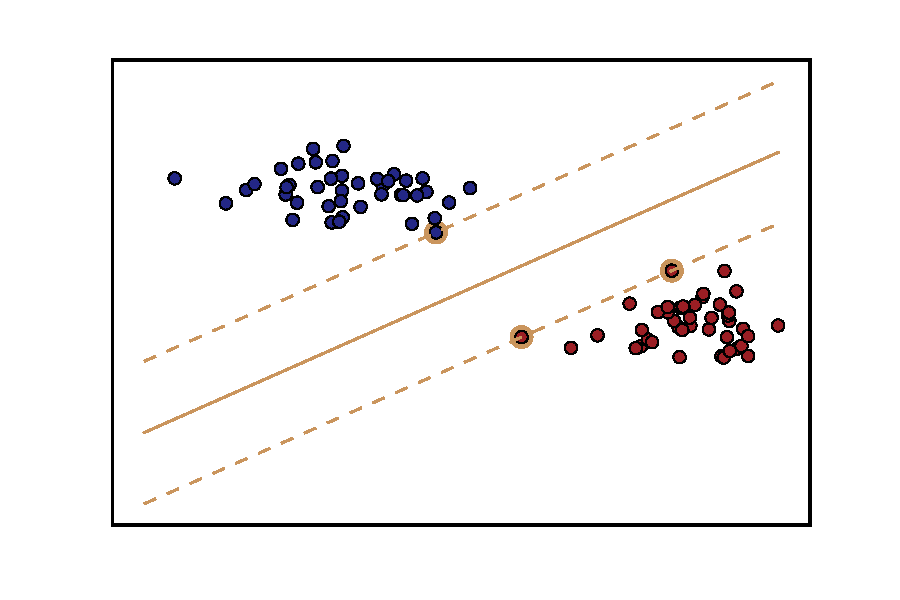
\includegraphics[width = \figwidth]{pics/ml/hyperplane_lin.pdf}
	\caption{The same points as those shown in figure \ref{fig:fisher_example}, except points in {\color{moerkeroed} class a} and {\color{oldhat} class b} are now pictured along with their {\color{nude} maximally separating hyperplane}.}
	\label{fig:separating_plane_example1}
\end{figure}
Using labels $\pm1$ to denote classes, the problem may be stated as trying to guess the mapping from an N-dimensional data space to classes $f: \mathbb{R}^N \rightarrow \cb{\pm1}$ based on a set of training data in $\mathbb{R}^N \otimes \cb{\pm1}$. I'll describe separately the properties of this maximally separating hyperplane, how it is obtained, and how the method is generalized to non-linear classification problems as the 'island' illustrated in figure~\ref{fig:island_example}.

The well-known equation for a plane is obtained by requiring that its normal vector $\mathbf{w}$ be orthogonal to the vector from some point in the plane $\mathbf{p}$ to any point $\mathbf{x}$ contained in it:
\begin{equation}
	\mb{w}\cdot\pp{\mb{x} - \mb{p}} = 0. \label{eqn:plan_simpel}
\end{equation}
The left hand side of \eqref{eqn:plan_simpel} gives zero for points in the plane and positive or negative values when the point is displaced in the same or opposite direction as the normal vector, respectively. Hence,  $\text{sign}\pp{\mb{w}\cdot\pp{\mb{x} - \mb{p}}}$ may be taken as the decision function. It is clear from \eqref{eqn:plan_simpel} that the normal vector may be scaled without changing the actual plane (of course the decision function is inverted if a negative value is chosen), so $\mb{w}$ is usually rescaled such that
\begin{equation}
	\mb{w}\cdot\pp{\mb{x} - \mb{p}} = \mb{w}\cdot \mb{x} + b = \pm 1, \label{eqn:rescaled_normal_vector}
\end{equation}
for the points that are closest to the separating plane. Those points located on the margin are encircled in figure \ref{fig:separating_plane_example1}. In general then, the meaning of the sign and magnitude of
\begin{equation}
	\mb{w}\cdot \mb{x} + b  \label{eqn:classification_decision_function}
\end{equation}
will be the predicted class and a measure of prediction confidence, respectively, for new data points. Finally, note that $\mb{w}$ can be expanded in terms of the data points that are on the margin in figure \ref{fig:separating_plane_example1} as
\begin{equation}
	\mb{w} = \sum_i v_i \mb{x}_i,
\end{equation}
these $\mb{x}_i$, the position vectors of the margin points in data space, are the 'support vectors' that lend their name to the method.

\subsection{Obtaining the Maximally Separating Hyperplane}
Assuming first that it is possible to slice the data space into two regions that contain only points corresponding to one class each, and that the plane's normal vector has already been rescaled according to \eqref{eqn:rescaled_normal_vector}, the following inequalities hold:
\begin{equation}
	\begin{aligned}
		\mb{x}_i\cdot \mb{w} + b &\ge 1, y_i = +1, \\
		\mb{x}_i\cdot \mb{w} + b &\le -1, y_i = -1.
	\end{aligned} \label{eqn:dedersenslagrangebetingelserder}
\end{equation}
Multiplying by $y_i$, both simply become
\begin{equation}
	y_i\pp{\mb{x}_i\cdot \mb{w} + b} - 1 \ge 0. \label{eqn:kombineret_lagrangeting}
\end{equation}
The distance between the separating plane and each of the margins in figure \ref{fig:separating_plane_example1} is $1/|\mb{w}|$, so in order to maximize the separation, $|\mb{w}|$ must be minimized. For mathematical convenience, $\frac{1}{2} |\mb{w}|^2$, rather than $|\mb{w}|$ is included in the Lagrangian, which then becomes
\begin{equation}
	L = \frac{1}{2} |\mb{w}|^2 - \sum_i \alpha_i y_i \pp{\mb{x}_i\cdot \mb{w} + b - 1}, \label{eqn:primal_lagrangian}
\end{equation}
must be minimized with the constraints
\begin{align}
	\alpha_i &\ge 0, \\
	\pardiff{L}{\alpha_i} &= 0.
\end{align}
A result from convex optimization theory known as Wolfe Duality\cite{wolfe1961duality} states that one may instead maximize the above Lagrangian subject to
\begin{equation}
	\nabla_w L = \pardiff{L}{b} = 0,
\end{equation}
which gives conditions
\begin{align}
	\mb{w} &= \sum_j \alpha_jy_j\mb{x}_j, \\
	\sum_j \alpha_jy_j &= 0.
\end{align}
These can be plugged back into \eqref{eqn:primal_lagrangian} to obtain
\begin{align}
	L_D &= \frac{1}{2} \sum_i \sum_j \alpha_i y_i \alpha_j y_j \mb{x}_i \cdot \mb{x}_j
	- \sum_i \alpha_i y_i \big( \mb{x}_i \cdot \sum_j \alpha_j y_j \mb{x}_j + b \big) + \sum_i \alpha_i, \\
	L_D &= -\frac{1}{2} \sum_{i,j} \alpha_i \alpha_j y_i y_j \mb{x}_i \mb{x}_j + \sum_i \alpha_i. \label{eqn:dual_lagrangian}
\end{align}
A problem with this is that eqs \ref{eqn:dedersenslagrangebetingelserder} can only be satisfied in the completely separable case, although it is easy to imagine an example in which a classifier performs well but not flawlessly on the training set. For instance, if two points, one from each class, in figure \ref{fig:separating_plane_example1} were permuted, the classifier shown in the plot would still do a very good job, but eqs. \ref{eqn:dedersenslagrangebetingelserder} would not be satisfiable, causing the method to fail. This is remedied by introducing slack variables\cite{Boyd2004}
\begin{align}
\begin{split}
		\mb{x}_i\cdot \mb{w} + b &\ge 1 - \xi_i,\quad y_i = +1, \\
		\mb{x}_i\cdot \mb{w} + b &\le -(1 - \xi_i),\quad y_i = -1, \\
		\xi_i &\ge 0,
\end{split} \label{eqn:slack_variables}
\end{align}
which allows the algorithm to misclassify. This should come without a cost to the overall Lagrangian, or one would just end up classifying randomly, so a 'cost term', $C\cdot\sum_i\xi_i$ is added as well. The value of $C$ (as well as a few similar parameters which have yet to be introduced) is usually determined experimentally by simply varying it across some space of possible values and choosing the value resulting in the best performance - see for instance figure \ref{fig:grid_search_gamma_c}. In the case of the misclassification cost parameter $C$, low values will result in low performance, whereas too large values will result in overfitting. The above can be rewritten exactly as previously, except another set of non-negative Lagrange multipliers $\mu_i$ are added to \eqref{eqn:primal_lagrangian} to ensure positivity of the $\xi_i$, resulting in
\begin{equation}
	L = \frac{1}{2} |\mb{w}|^2 + C\cdot \sum_i\xi_i - \sum_i \alpha_i y_i \pp{\mb{x}_i\cdot \mb{w} + b - 1 + \xi_i} - \sum_i\mu_i\xi_i. \label{eqn:langgrimlagrangian}
\end{equation}
This results in the same dual Lagrangian $L_D$ as before, but with an upper bound on the $\alpha_i$:
\begin{equation}
	0 \le \alpha_i \le C.
\end{equation}
% Nopenopenopenope
%\begin{figure}
%	\centering
%	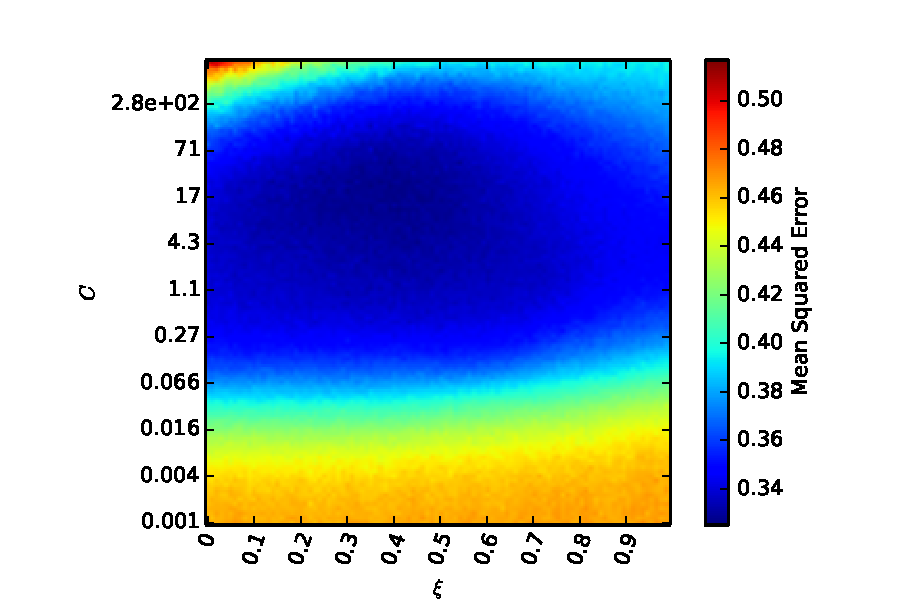
\includegraphics[width = \figwidth]{pics/ml/grid_search_svr_e_logc.pdf}
%	\caption{Heat map of the result of a grid search over the parameter space of the variables $\xi$ and $C$. The colors signify the mean squared error of a support vector regression problem, which is closely related to the classification problem described in the present section. Note how overfitting damages performance for high values of $C$. The minimum MSE was obtained using $C=26.5$ and $\xi=0.11$.}
%	\label{fig:grid_search_heatmap}
%\end{figure}
The methods outlined above can also be used to solve regression, rather than classification, problems\cite{Smola2004}. The training data will then be in $\mathbb{R}^{N+1}$ rather than in $\mathbb{R}^N \otimes \cb{\pm1}$, and the value of the decision function in \eqref{eqn:classification_decision_function} is predicted instead of using only its sign. The criterion of correct classification from \eqref{eqn:kombineret_lagrangeting} is replaced by the demand that predictions be within some tolerated margin $\epsilon$ of the true value of the training point $y_i$, so \eqref{eqn:dedersenslagrangebetingelserder} becomes
\begin{equation}
	-\epsilon \leq \mb{x}_i\cdot\mb{w} + b - y_i \leq \epsilon
\end{equation}
so when slack variables $\xi_i$ and $\xi^{*}_i$ (for the lower and upper bound, respectively) like in \eqref{eqn:slack_variables} are introduced, the Lagrangian from \eqref{eqn:langgrimlagrangian} becomes
\begin{equation}
	L = \frac{1}{2} |\mb{w}|^2 + C \sum_{i}\pp{\xi_i + \xi^{*}_i},
\end{equation}
with constraints
\begin{align}
	\mb{x}_i\cdot\mb{w} + b - y_i &\geq -\pp{\epsilon + \xi_i}, \\
	\mb{x}_i\cdot\mb{w} + b - y_i &\leq \epsilon + \xi^{*}_i, \\
	\xi_i, \xi^{*} &\geq 0.
\end{align} 


The main point to be emphasized here is that the training data $\mb{x}_i$ only enter into the dual Lagrangian of \eqref{eqn:dual_lagrangian} as inner products. This is essential when extending the SVM model to nonlinear cases, which is the subject of the following section.

\subsection{Generalizing to the non-linear case}
\label{sec:svm_nonlinear}
The fact that the data $\mb{x}_i$ only occur as inner products in \eqref{eqn:dual_lagrangian} makes one way of generalizing to non-linearly separable datasets straightforward: Referring back to figure \ref{fig:island_example}, one might imagine bending the plane containing the data points by curling the edges outwards in a third dimension after which a two-dimensional plane could separate the points very well. In general, this means applying some mapping
\begin{equation}
	\Phi: \mathbb{R}^l \to \mathbb{R}^h, \quad h > l,
\end{equation}
to the $\mb{x}_i$ ($l$ and $h$ are for low and high, respectively). For example, one could look for a mapping such that the new inner product becomes
\begin{equation}
	\Phi(\mb{x}_i) \cdot\Phi(\mb{x}_j) = \pp{\mb{x}_i\cdot \mb{x}_j}^2. 
\end{equation}
I'll describe the components of each vector separately, so I'm going to change notation to let the subscripts denote coordinates and using $\mb{x}$ and $\mb{y}$ as two arbitrary feature vectors, where the latter shouldn't be confused with the class labels used earlier. As an example, in two dimensions the above becomes
\begin{equation}
	\pp{\mb{x} \cdot \mb{y}}^2 = \pp{\sum_{i=1}^2 x_i y_i}^2 = x_1^2 y_1^2 + 2x_1y_1x_2y_2 + x_2^2 y_2^2,
\end{equation}
meaning that one possibility for $\Phi$ is
\begin{equation}
	\Phi: \mb{x} \mapsto \begin{pmatrix} x_1^2 \\ \sqrt{2}x_1x_2 \\ x_2^2 \end{pmatrix}
\end{equation}
This can be generalized to $d$-dimensional feature vectors and to taking the $n$'th power rather than the square using the multinomial theorem:
\begin{equation}
	\pp{\sum_{i=1}^d x_i}^n = \sum_{\sum_{i=1}^d k_i = n} \frac{n!}{\prod_{l=1}^d k_l!} \prod_{j = 1}^d x_j^{k_j}, \label{eqn:multinomial_raw}
\end{equation}
where the subscript $\sum_{i=1}^d k_i = n$ simply means that the sum goes over any combination of $d$ non-negative integers $k_i$ that sum to $n$. I wish to rewrite this slightly for two reasons: to simplify the notation in order to make a later proof more manageable, and to help quantify how quickly the number of dimensions in the output space grows to motivate a trick to avoid these explicit mappings.

As stated, the sum on the RHS of \eqref{eqn:multinomial_raw} runs over all combinations of $d$ integers which sum to $n$.
This can be simplified by introducing a function $K$, which simply maps
\begin{equation}
	K: n,d \mapsto \cb{\cb{k} \in \mathbb{N}^d \left| \sum_{i=1}^d k_i = n \right.}, 
\end{equation}
and denoting each of those collections $\cb{k}_i$ so each of the coefficients in \eqref{eqn:multinomial_raw} can be written
\begin{equation}
	\frac{n!}{\prod_{i=1}^dk_i!} = C_{\cb{k}}.
\end{equation}
Then, \eqref{eqn:multinomial_raw} becomes
\begin{equation}
	\pp{\sum_{i=1}^d x_i}^n = \sum_{K(n,d)} C_{\cb{k}} \prod_{j = 1}^d x_j^{k_j} \label{eqn:multinomial_smart}
\end{equation}
To show how quickly the dimensions of the required embedding space grows, note that the dimension is equal to the number of terms in the sum above, i.e.
\begin{equation}
	\mathrm{dim}(\mathbb{R}^h) = \left| K(n,d) \right| = \left| \cb{\cb{k} \in \mathbb{N}^d \left| \sum_{i=1}^d k_i = n \right.} \right|,
\end{equation}
which can be computed using a nice trick known from enumerative combinatorics.

Consider the case where $n=5$ and $d=3$. $K(5,3)$ then contains all sets of 3 integers summing to 5, such as $1,3,1$ or $0,1,4$. Each of these can be uniquely visualized as 5 unit values distributed into 3 partitions in the following fashion:
\begin{align*}
	\circ~|~\circ~\circ~\circ~|~\circ, \\
	|~\circ~|~\circ~\circ~\circ~\circ,
\end{align*}
and so on. It should be clear that you need $n$ $\circ$-symbols and $d-1$ $|$ separators. The number of possible such combinations, and hence the dimensionality of the embedding space, is then
\begin{equation}
	\begin{pmatrix}
		n + d - 1 \\ n
	\end{pmatrix}
	= \frac{(n+d-1)!}{n!(d-1)!}.
\end{equation}
This number quickly grows to be computationally infeasible, which motivates one to look for a way to compute the inner product in the embedded space without performing the explicit mapping itself. This is the point of the so-called 'kernel trick', which I'll introduce in the following.

The idea of the kernel trick is that since only the inner products between feature vectors in the embedded space are required, one might as well look for some function $K$ of the original feature vectors which gives the same scalar as the inner product in the embedded space, i.e.
\begin{equation}
	K(\mb{x}, \mb{y}) = \Phi(\mb{x}) \cdot \Phi(\mb{y}). \label{eqn:kernel_basic}
\end{equation}
In the polynomial case treated above, the correspondence between the kernel function $K(\mb{x}, \mb{y})$ and the explicit mapping $\Phi$ is straightforward:
\begin{align}
	K(\mb{x}, \mb{y}) &= \pp{\mb{x} \cdot \mb{y}}^n, \\
	\Phi(\mb{x}) &= \sum_{K(n,d)} \sqrt{C_{\cb{k}}} \prod_{j = 1}^d x_j^{k_j},
\end{align}
so that \eqref{eqn:kernel_basic} is true by the multinomial theorem and the above considerations. However, situations arise
% Becaaaause of the weeeaather!
in which the explicit mapping $\Phi$ isn't directly obtainable, and the correspondence of the kernel function to inner products in higher dimensional spaces is harder to demonstrate. This is the subject of the following section.

\subsubsection{Radial Basis Functions}
One commonly used kernel function is the RBF, or radial basis function, kernel:
\begin{equation}
	K(\mb{x}, \mb{y}) = \e^{|\mb{x}-\mb{y}|^2/2\sigma}. \label{eqn:rbf_kernel}
\end{equation}
Burges \cite{burges1998} shows that the polynomial kernel is valid, so I'll show how the argument extends to the RBF kernel in the following.

Mercer's condition\cite{Smola1998} states that for a kernel function $K(\mb{x}, \mb{y})$, there exists a corresponding Hilbert space $\mathcal{H}$ and a mapping $\Phi$ as specified earlier, iff any $L^2$-normalizable function $g(\mb{x})$ satisfies
\begin{equation}
	\int K(\mb{x}, \mb{y}) g(\mb{x}) g(\mb{y}) \ud\mb{x} \ud\mb{y} \ge 0. \label{eqn:mercers_condition}
\end{equation}
This can be shown be rewriting \eqref{eqn:rbf_kernel} as
\begin{equation}
	K(\mb{x}, \mb{y}) = \e^{(\mb{x}-\mb{y})\cdot(\mb{x}-\mb{y})/2\sigma} = \e^{|\mb{x}|^2/2\sigma} \e^{|\mb{y}|^2/2\sigma} \e^{-\mb{x}\cdot\mb{y}/\sigma}, \label{eqn:grimligningsomjegaldrigkommertilatbrugeigen}
\end{equation}
and expanding the last term in $(\mb{x}\cdot\mb{y})$ as
\begin{equation}
	\e^{-\mb{x}\cdot\mb{y}/\sigma} = \sum_{i=0}^\infty \frac{(-1)^i}{i!\sigma^i} \pp{\mb{x}\cdot\mb{y}}^i,
\end{equation}
but using \eqref{eqn:multinomial_smart} on the dot product gives
\begin{equation}
	\pp{\mb{x}\cdot\mb{y}}^i = \pp{\sum_{j=1}^d x_j y_j}^i = \sum_{K(i,d)} C_{\cb{k}} \prod_{j = 1}^d x_j^{k_j} y_j^{k_j}
\end{equation}
so the Taylor expansion becomes
\begin{equation}
	\e^{-\mb{x}\cdot\mb{y}/\sigma} = \sum_{i=0}^\infty \sum_{K(i,d)} \frac{(-1)^i}{i!\sigma^i}  C_{\cb{k}}  \prod_{j = 1}^d x_j^{k_j} y_j^{k_j},
\end{equation}
which can be plugged back into \eqref{eqn:grimligningsomjegaldrigkommertilatbrugeigen} to yield
\begin{equation}
	K(\mb{x}, \mb{y}) = \sum_{i=0}^\infty \sum_{K(i,d)} \frac{(-1)^i}{i!\sigma^i}  C_{\cb{k}} \e^{|\mb{x}|^2/2\sigma} \e^{|\mb{y}|^2/2\sigma} \prod_{j = 1}^d x_j^{k_j} y_j^{k_j}. \label{eqn:ehrmagehrditsseparable}
\end{equation}
The underlying reason for these algebraic shenanigans is that \eqref{eqn:ehrmagehrditsseparable} is clearly separable so that the integral in \eqref{eqn:mercers_condition} from Mercer's condition becomes
\begin{align}
	& \int K(\mb{x}, \mb{y}) g(\mb{x}) g(\mb{y}) \ud\mb{x} \ud\mb{y} \\
	 = & \sum_{i=0}^\infty \sum_{K(i,d)} \frac{(-1)^i}{i!\sigma^i}  C_{\cb{k}} \int_{\mathbb{R}^{2d}} \e^{|\mb{x}|^2/2\sigma} \e^{|\mb{y}|^2/2\sigma} \prod_{j = 1}^d x_j^{k_j} y_j^{k_j} g(\mb{x}) g(\mb{y}) \ud\mb{x}\ud\mb{y} \\
	= &\sum_{i=0}^\infty \sum_{K(i,d)} \frac{(-1)^i}{i!\sigma^i}  C_{\cb{k}} \left(\int_{\mathbb{R}^{d}} \e^{|\mb{x}|^2/2\sigma} \prod_{j = 1}^d x_j^{k_j} g(\mb{x}) \ud\mb{x} \right)\cdot
	  \left(\int_{\mathbb{R}^{d}} \e^{|\mb{y}|^2/2\sigma} \prod_{j = 1}^d y_j^{k_j} g(\mb{y}) \ud\mb{y} \right) \\
	= &\sum_{i=0}^\infty \sum_{K(i,d)} \frac{(-1)^i}{i!\sigma^i}  C_{\cb{k}} \left(\int_{\mathbb{R}^{d}} \e^{|\mb{x}|^2/2\sigma} \prod_{j = 1}^d x_j^{k_j} g(\mb{x}) \ud\mb{x} \right)^2 \\
	\ge & 0.
\end{align}
Hence, radial basis functions satisfy Mercer's condition and the kernel described above can be plugged into the dual Lagrangian from \eqref{eqn:dual_lagrangian} to obtain
\begin{equation}
	L_D = -\frac{1}{2} \sum_{i,j} \alpha_i \alpha_j y_i y_j \e^{|\mb{x}_i-\mb{x}_j|^2/2\sigma} + \sum_i \alpha_i,
\end{equation}
which must be maximized subject to the same constraints as earlier. The concrete optimization procedure is complicated and already implemented in most machine learning libraries, so I choose not to go into details with that, but instead to demonstrate the effectiveness of the RBF kernel approach on the non-linear-separable points that were generated earlier. figure~\ref{fig:kernel_trick_example} shows the points again, along with the \textit{decision frontier} i.e. the curve which separates regions in which points are classified into separate classes.
\begin{figure}
	\centering
	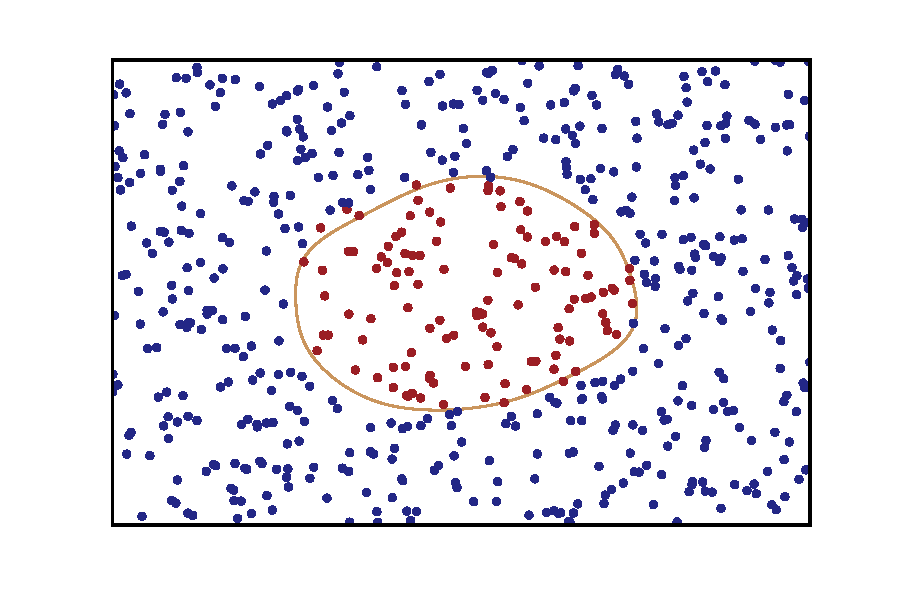
\includegraphics[width = \figwidth]{pics/ml/kernel_example.pdf}
	\caption{The 'island' scenario of figure \ref{fig:island_example} revisited. The points representing {\color{moerkeroed} class a} and {\color{oldhat}class b} have been mapped to a higher-dimensional space in which it is possible to construct a separating hyperplane whose {\color{nude} decision frontier} is also shown.}
	\label{fig:kernel_trick_example}
\end{figure}
The danger of overfitting should be clear from figure \ref{fig:kernel_trick_example}. If the cost of misclassification $C$ and the sharpness of the RBFs, usually denoted by $\gamma=2/\sigma$ are set sufficiently high, the algorithm will simply end up with a tiny decision boundary around every training point of class a, resulting in flawless classification on the training set, but utter failure on new data.
The typical way of evaluating this is to perform k-fold validation, meaning that the available data is $k$ equal parts and the SVM is consecutively trained on $k-1$ parts and tested on the remaining. A variant of this, which my code uses, is stratified k-fold validation, which only differs in that the data is partitioned so as to keep the ratio between the different classes in each parts as close to equal as possible.

The $\gamma$ parameter is often fixed by performing a grid search similar to that discussed earlier. Figure \ref{fig:grid_search_gamma_c} shows the resulting heat map from a grid search.
\begin{figure}
	\centering
	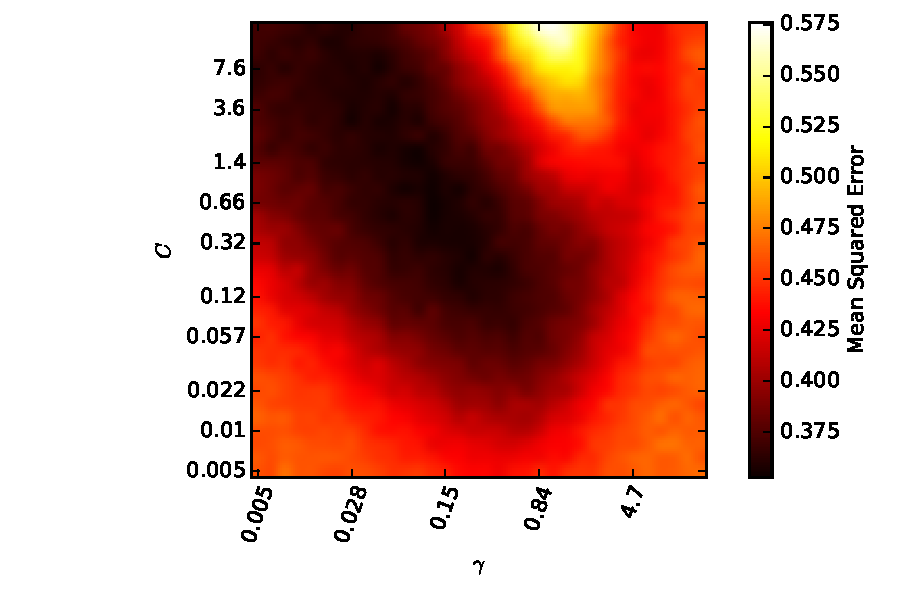
\includegraphics[width = \figwidth]{pics/ml/15_07_20_grid_search_g_thr_extra.pdf}
	\caption{Result of a grid search for the optimal combination of values for the cost parameter $C$ and the sharpness $\gamma$ of the Gaussian kernel function giving optimal values of $C = 0.52$ and $\gamma = 0.12$.}
	\label{fig:grid_search_gamma_c}
\end{figure}

\FloatBarrier
\subsection{Implementing a custom weighted radial basis function kernel}
In general, the features extracted as described in section \ref{sec:data_extraction} are too numerous for efficient implementations of most machine learning schemes. \cite{demontjoye2013} work around this by determining the linear correlation between each feature and the target values, and then discarding features whose correlation is below some threshold and letting the rest contribute equally in the SVM. They never explicate this threshold but state that they include features 'significantly related' to the target values, which convention would suggest means a threshold of $0.05$. \cite{Pietersma2011} have demonstrated significant improvements in SVM performance by assigning variable importances to each feature, so I implemented a modified kernel function where I don't just discard features with linear correlations below some threshold but also assign to each remaining feature a normalized weight given by its correlation with the output variable.

I do this by defining a diagonal matrix $\hat{M}$ where the $i, i$th element is the linear correlation coefficient between feature $i$ and the target variable, and using the matrix as a metric in the exponent of the usual radial basis functions so the kernel $K(\mb{x}, \mb{y})$ becomes
\begin{equation}
	\e^{\gamma|\mb{x}-\mb{y}|^2} \rightarrow \e^{\gamma \pp{\mb{x}-\mb{y}}^T \hat{M} \pp{\mb{x}-\mb{y}}}
\end{equation}
Note that this does not change the validity of the proof I gave in section \ref{sec:svm_nonlinear}, so this weighted RBF kernel also satisfies Mercer's condition and may hence be used as a kernel function. It turned out to be nontrivial to write an implementation of this which had a syntax consistent with that of the default methods available in the library I used, and which provided a similarly simple way to grid search over its parameters ($C$ and $\gamma$ as in the usual RBF kernel SVM along with a threshold parameter). I ended up solving this by writing a metamethod to provide a kernel matrix based on an input list of variable importances as well as a default sharpness parameter denoted $\gamma$.
\begin{snippet}
	def make_kernel(importances, gamma = 1.0):
		'''Returns a weighted radial basis function (WRBF) kernel which can be 
		passed to an SVM or SVR from the sklearn module.
		
		Parameters:
		-----------------------
		importances : list
		  The importance of each input feature. The value of element i can mean
		  e.g. the linear correlation between feature i and target variable y.
		  None means feature will be weighted equally.
		
		gamma : float
		  The usual gamma parameter denoting inverse width of the gaussian used.
		'''
		def kernel(x,y, *args, **kwargs):
			d = len(importances)  #number of features
			impsum = sum([imp**2 for imp in importances])
			if not impsum == 0:
				normfactor = 1.0/np.sqrt(impsum)
			else:
				normfactor = 0.0
			#Metric to compute distance between points
			metric = dok_matrix((d,d), dtype = np.float64)
			for i in xrange(d):
				metric[i,i] = importances[i]*normfactor
			# 
			result = np.zeros(shape = (len(x), len(y)))
			for i in xrange(len(x)):
				for j in xrange(len(y)):
					diff = x[i] - y[j]
					dist = diff.T.dot(metric*diff)
					result[i,j] = np.exp(-gamma*dist)
			return result
		return kernel
\end{snippet}
With that in place, it was a simple matter to implement classifiers and regressors by inheriting from the default classes and overriding the constructor methods like this:
\begin{snippet}
	class WRBFR(svm.SVR):
		'''Weighted radial basis function support vector regressor.'''
		def __init__(self, importances, C = 1.0, epsilon = 0.1,
				      gamma = 0.0):
		kernel = make_kernel(importances = importances, gamma = gamma)
		super(WRBFR, self).__init__(C = C, epsilon = epsilon, kernel = kernel)
\end{snippet}
Figures \ref{fig:grid_thr_g} and \ref{fig:grid_thr_c} show heat maps resulting from grid searches over the threshold parameter versus $\gamma$ and $C$, respectively. Interestingly, the ideal correlation threshold seems to be well above the value used in \cite{demontjoye2013}.
\begin{figure}
	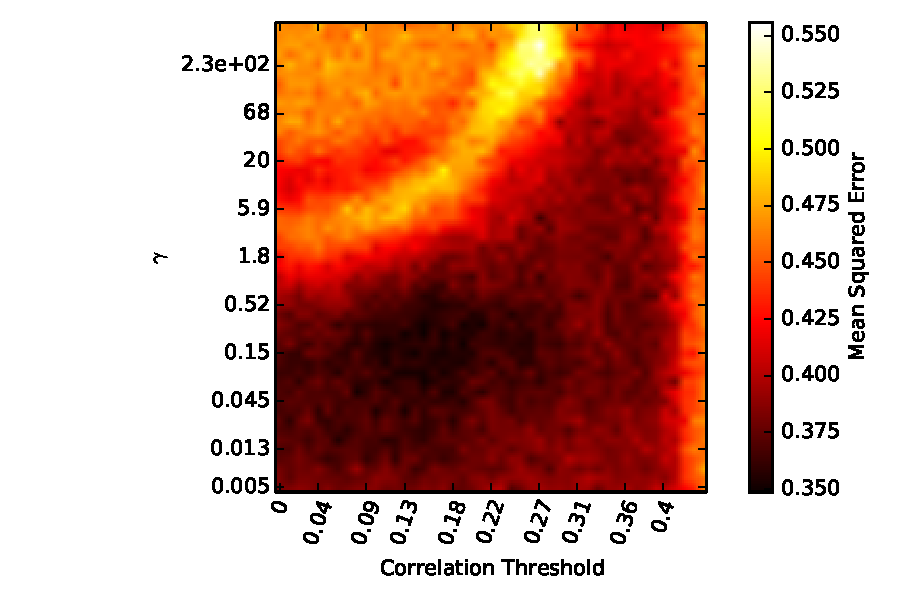
\includegraphics[width=\figwidth]{pics/ml/15_07_17_grid_search_g_thr_extra.pdf}
	\caption{Heat map resulting from a grid search over the parameter space of the linear correlation threshold and the default sharpness $\gamma$ of the radial basis functions showing optimal values of $0.25$ and $0.15$ for $\gamma$ and the threshold, respectively.}
	\label{fig:grid_thr_g}
\end{figure}

\begin{figure}
	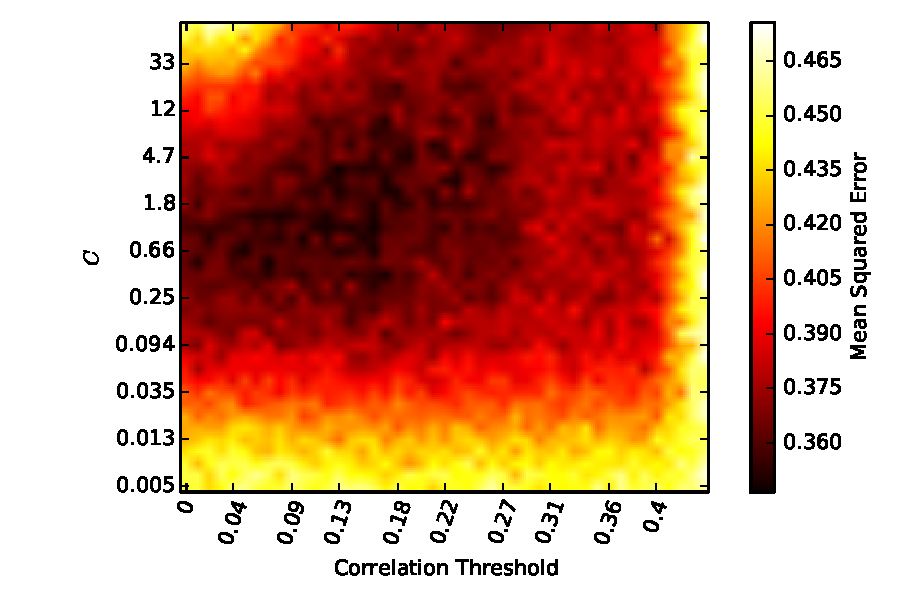
\includegraphics[width=\figwidth]{pics/ml/15_07_15_grid_search_c_thr_extra.pdf}
	\caption{Heat map resulting from a grid search over the parameter space of the linear correlation threshold and the cost parameter $C$ of the radial basis functions showing optimal values of $3.6$ and $0.13$ for $\gamma$ and the threshold, respectively.}
	\label{fig:grid_thr_c}
\end{figure}





\FloatBarrier
\subsection{Statistical subtleties}
% http://www.visiondummy.com/2014/03/divide-variance-n-1/
An important note should be made here about some often neglected subtleties relating to uncertainties. Physicists often deal with measurements that can assumed to be independently drawn from a normal distribution $\mathcal{N}(x_i;\mu, \sigma^2)$ due to the central limit theorem. With a large number of measurements $n$, the standard deviation of a sample
\begin{equation}
	\sigma^2 = \frac{1}{N}\sum_i^N \pp{x_i - \mu}^2,
\end{equation}
converges as $N \rightarrow \infty$ to the maximum likelihood, minimum variance unbiased estimator for the true variance of the underlying distribution with unknown mean
\begin{equation}
	\hat{\sigma}^2 = \frac{1}{N-1} \sum_i^N \pp{x_i - \mu}^2.
\end{equation}
The standard deviation $\sigma$ and the width of the underlying gaussian $\hat{\sigma}^2$ can then often be used interchangeably. This tempts some people into the questionable habit of always assuming that the sample standard deviance can be used as the $68\%$ confidence interval of their results.

When using a K-fold validation scheme, the performance scores for the various folds cannot be assumed to be independently drawn from an underlying distribution, as the test set of one fold is used in the training sets of the remaining folds. In fact, it has been shown \cite{Bengio2004} that there is no unbiased estimator for the variance of the performance estimated using K-fold validation. However, as K-fold validation is more effective than keeping the test, and training data separate, which can be shown using Jensen's inequality along with some basic properties of expectation values \cite{Blum1999}, I'll mostly use K-fold regardless. As the standard deviation still provides a qualitative measure of the consistency of the model's performance, I'll still use the sample STD in a usual fashion, such as error bars, unless otherwise is specified, but the reader should keep in mind that these do not indicate precise uncertainties whenever K-fold validation has been involved.

\section{Decision Trees \& Random Forests}
Another popular machine learning scheme is that of random forests, which consist of an ensemble of decision trees.
A decision tree is a very intuitive method for classification problems which can be visualized as a kind of flow chart in the following fashion. As usual, the problem consists of a set of feature vectors $\mb{x}_i$ and a set of corresponding class labels $y_i$. A decision tree then resembles a flowchart starting at the root of the tree, at each node splitting into branches and finally branching into leaves at which all class labels should be identical. At each node, part of the feature vector is used to split the dataset into parts. This resembles the 'twenty questions' game, in which one participant thinks of a famous person and another attempts to guess who it is by asking a series of yes/no-questions, each one splitting the set of candidates in two parts. In this riddle game and in decision tree learning, there are good and bad questions (asking whether the person was born on March 14th, 1879 is a very bad first question, for instance). There are several ways of quantifying how 'good' a yes/no-question, corresponding to a partitioning of the dataset, is.

On metric for this is the Gini Impurity Index $I_G$, which is computed by summing over each class label:
\begin{equation}
	I_G = \sum_i f_i \pp{1-f_i} = 1 - \sum_i f_i^2,
\end{equation}
where $f_i$ denotes the fraction of the set the consists of class $y_i$. Using this as a metric, the best partitioning is the one which results in the largest drop in total Gini impurity following a branching.
Another metric is the information gain measured by comparing the entropy before a split with a weighted average of the entropy in the groups resulting from the split. Denoting the fractions of the various classes in the parent group, i.e. before splitting, by $f_i$ and the two child groups by $a_i$ and $b_i$, the information gain is
\begin{equation}
	I_E = -\sum_i f_i \log_2 f_i + \frac{n_a}{N} \sum_i a_i \log_2 a_i + \frac{n_b}{N} \sum_i b_i \log_2 b_i.
\end{equation}

However, if too many such nodes are added to a decision tree, overfitting, i.e. extreme accuracies on training data but poor performance on new data, becomes a problem. This can be remedied by instead predicting with a majority vote, or averaging in the case of regression problems, from an ensemble of randomized decision trees called a random forest. The main merits of random forests are their accuracy and ease of use, and their applications as auxiliary methods in other machine learning schemes, which I'll elaborate on shortly.

The individual trees in a random forest are grown using a randomly selected subset of the training data for each tree. The data used to construct a given tree is referred to as 'in bag', whereas the remaining training data is referred to as 'out of bag' (OOB) for the given tree. At each node, a set number of features is randomly selected and the best possible branching, cf. the above considerations, is determined. The only parameters that must be tweaked manually are the number of trees in the forest, number of features to include in each branching, and the maximum tree depth. While other variables such as the metric for determining branching quality as described above, may be customized, those aren't essential to achieve a decent predictor, which is robust in regard to both overfitting and irrelevant parameters.\cite{Breiman2001}

There doesn't seem to be a single universally accepted way of adjusting these parameters, so I chose a somewhat pragmatic approach of simply checking how well various choices for each parameter performed on a randomly selected trait. For instance, figure \ref{fig:determine_max_features} shows how well a random forest predicted the tertiles of participants' extroversion as a function of the fraction of available features each tree was allowed to include in each branching. This was done using a large number of trees ($n = 1000$) and using each of the two metrics described earlier.
\begin{figure}
	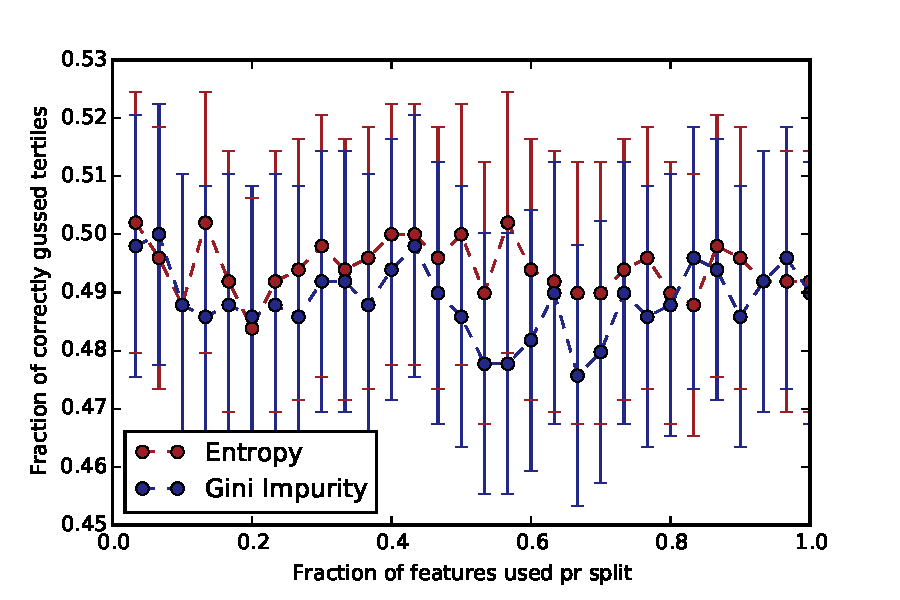
\includegraphics[width=\figwidth]{pics/ml/max_features_pr_split.pdf}
	\caption{Performance of a random forest with 1000 decision trees using various fractions of the available features in each branching using both the {\color{moerkeroed}entropy} and the {\color{oldhat}Gini impurity} metric to determine the optimal branching. The number of features seems not to play a major role, and the {\color{moerkeroed}entropy} metric seems to perform slightly better in general.}
	\label{fig:determine_max_features}
\end{figure}
The number of features used pr split doesn't seem to have any significant effect on performance, and as the entropy metric seems to perform as well or slightly better than Gini impurity, I decided to stick to that. A similar plot of the performance of various numbers of decision trees in the forest is shown in figure \ref{fig:determine_ntrees}.
\begin{figure}
	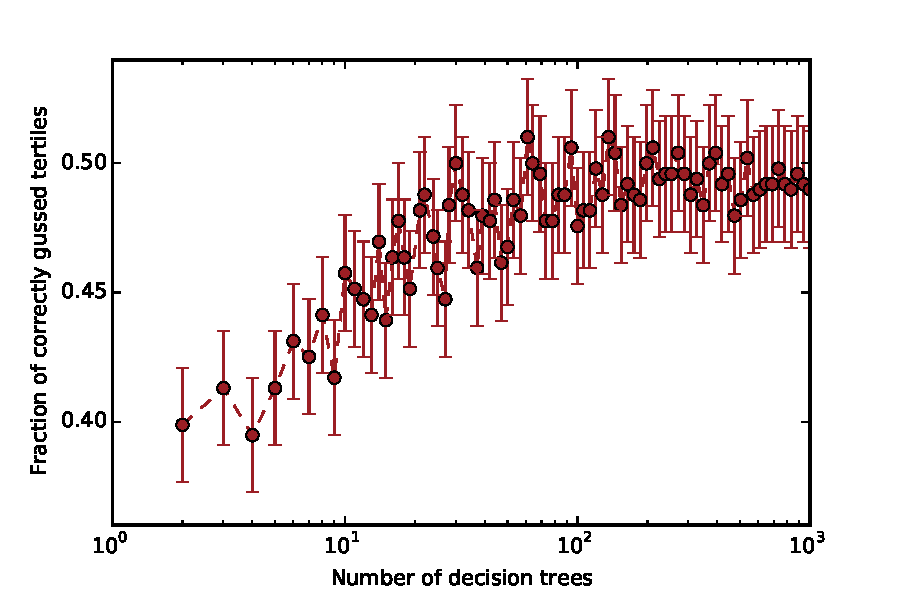
\includegraphics[width=\figwidth]{pics/ml/determine_ntrees.pdf}
	\caption{Example of a random forest performance versus number of decision trees. Performance seems to increase steadily until about 100 trees, then stagnate.}
	\label{fig:determine_ntrees}
\end{figure}
The performance seems to stagnate around 100 trees, and remain constant after that, so I usually used at least 500 trees to make sure to get the optimal performance, as runtime wasn't an issue.

The robustness to irrelevant features and overfitting described earlier also plays a role in the application of random forests in conjunction with other schemes. SVMs as described in section \ref{sec:svm} can be sensitive to irrelevant data\cite{Pietersma2011}. There exist off-the-shelf methods, such as recursive feature elimination (RFE)\cite{Guyon2002}, for use with linear SVMs, but to my knowledge, there is no 'standard' way to eliminate irrelevant features when using a non-linear kernel. However, it is possible to use a random forest approach to obtain the relative importance of the various features and then use only the most important ones in another machine learning scheme which is less tolerant to the inclusion of irrelevant data. The relative importance of feature $j$ can be estimated  by first constructing a random forest and evaluating its performance $s$, then randomly permuting the values of feature $j$ across the training sample and measure the damage it does to the performance of the forest by comparing with the permuted score $s_p$. The ratio of the mean to standard deviation of those differences:
\begin{equation}
	w_j = \frac{\langle s-s_p \rangle}{\mathrm{std}(s - s_p)}
\end{equation}	


Random forests also provide a natural measure of similarity between data points. Given data points $i$ and $j$ these can be plugged into all their OOB decision trees, or a random subset thereof, and the fraction of the attempts in which both end up at the same leaf can be taken as a measure of similarity. This can be used to generate a proximity matrix for the data points, and it can be used as a metric for determining the nearest neighbours of a new point in conjunction with a simple nearest neighbour classifier.

\section{Nearest Neighbour-classifiers}
Skriv en masse om den smart random forest NN-model. \todo{Do iiit!}


\section{Results}

\subsection{Big Five Personality Traits}
\FloatBarrier
HARJ
\begin{figure}
	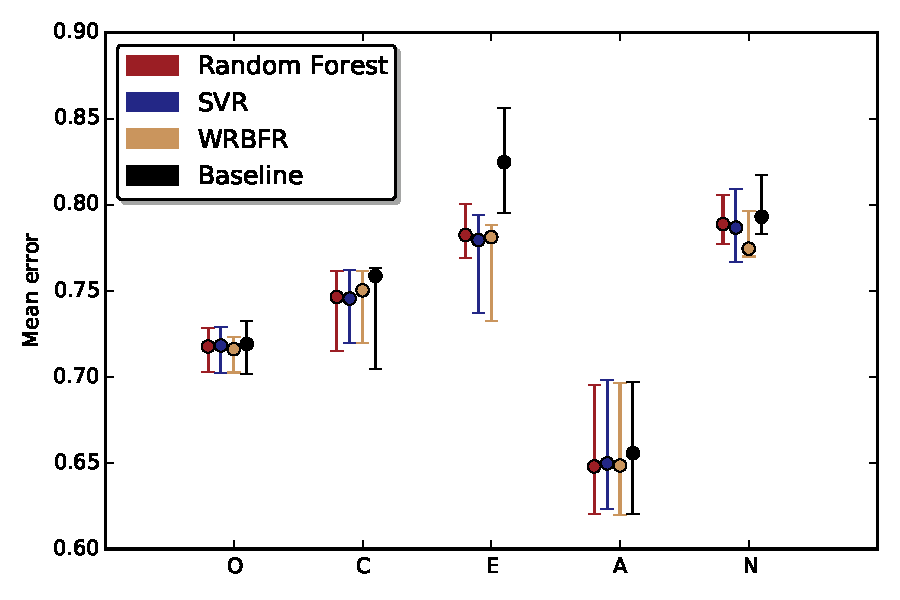
\includegraphics[width=\figwidth]{pics/ml/ml_cross_val_results.pdf}
	\caption{Comparison of performance of models using {\color{moerkeroed}random forest}, {\color{oldhat}support vector regression} and {\color{nude} weighted radial basis function regressor} with a {\color{black} \textbf{baseline model}} which always predicts the mean of the training sample. The y axis shows the mean error of each model and the error bars show the $95$-percentile around the median scores obtained by running on 1000 bootstrap samples.}
	\label{fig:cross_val_fail}
\end{figure}

\FloatBarrier
\subsection{Miscellaneous Traits}
Her står der ting om figur \ref{fig:correlation_grid}. \todo{Opdater med ML}
\begin{figure}
	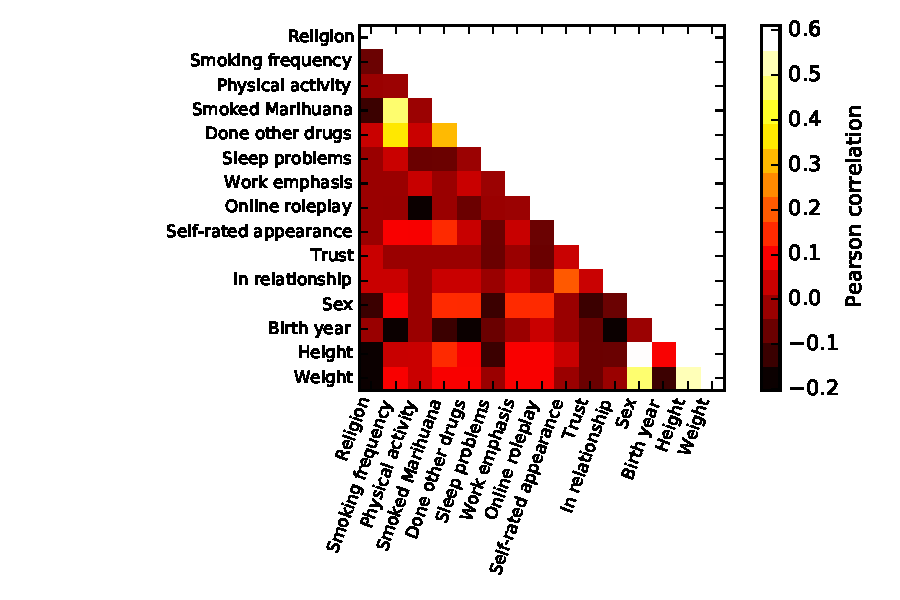
\includegraphics[width=\figwidth]{pics/ml/correlation_grid.pdf}
	\caption{Triangle of Pearson correlation coefficients for various miscellaneous traits.}
	\label{fig:correlation_grid}
	\end{figure}